\section{Computer Science Paper Results}

\subsection{Model simulation}

Using the influenza parameters of Table \ref{tab_params}, we simulated an infection initiated with 1001365 cells in a dish, an MOI of $10^{-4}$, and no initial virus. Figure \ref{fig_FullDish_cellandvirus} shows different views of plaques forming in the entire dish. On the left are cells in the different stages of infection described in section \ref{ABM}, where the healthy cells are colored green, eclipse cells are colored cyan, infected cells are colored red, and dead cells are colored black. On the right are figures showing the corresponding virus concentrations that are over the cells, where areas of higher concentration are colored yellow and areas of lower concentration are colored purple. Figure \ref{fig_FullDish_cellandvirus} shows the infection in 5 hour increments starting at 5 hours, when no cells are producing virus, and ending at 60 hours, when almost all the cells have died. The ABM reproduces the plaques typically seen in experimental \emph{in vitro} infections \cite{holder11H274Y}. 

For a closer look at the plaques, figure \ref{fig_ZoominDish} is a zoomed in view of the infection at hours 6.5, 11.5, and 16.5. The cells are shown on the left, with the same color scheme used in figure \ref{fig_FullDish_cellandvirus}, and the corresponding virus distribution is shown on the right. Here we can clearly see the heterogeneous growth of the plaque; it is not simply a radially symmetric change of cells from eclipse to infectious. 

\begin{figure}
\centering
\begin{minipage}{0.8\linewidth}
\centering
\begin{multicols}{2}
    \resizebox{0.48\textwidth}{!}{%
        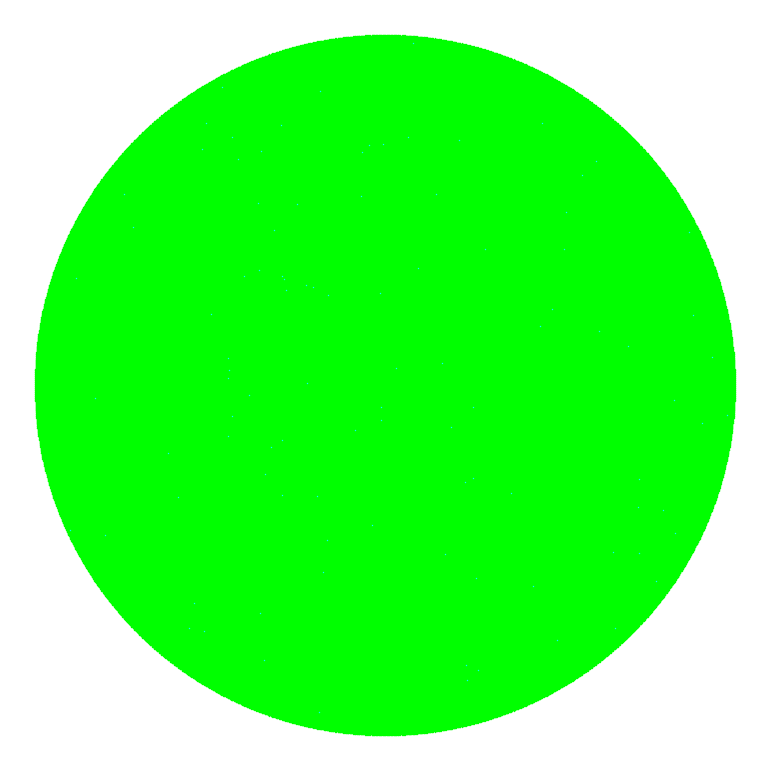
\includegraphics[width=0.48\textwidth]{Figures/Full-Dish-CellPhotos/cell9.png}
        
\includegraphics[width=0.48\textwidth]{Figures/Full-Dish-VirusPhotos/virus9.png}}

    \resizebox{0.48\textwidth}{!}{%
        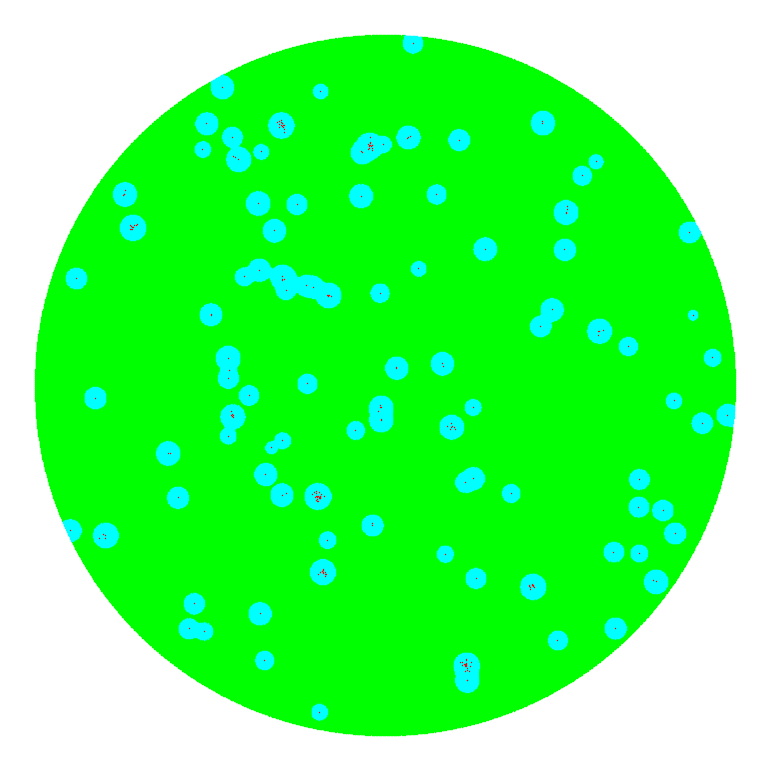
\includegraphics[width=0.48\textwidth]{Figures/Full-Dish-CellPhotos/cell19.png}
        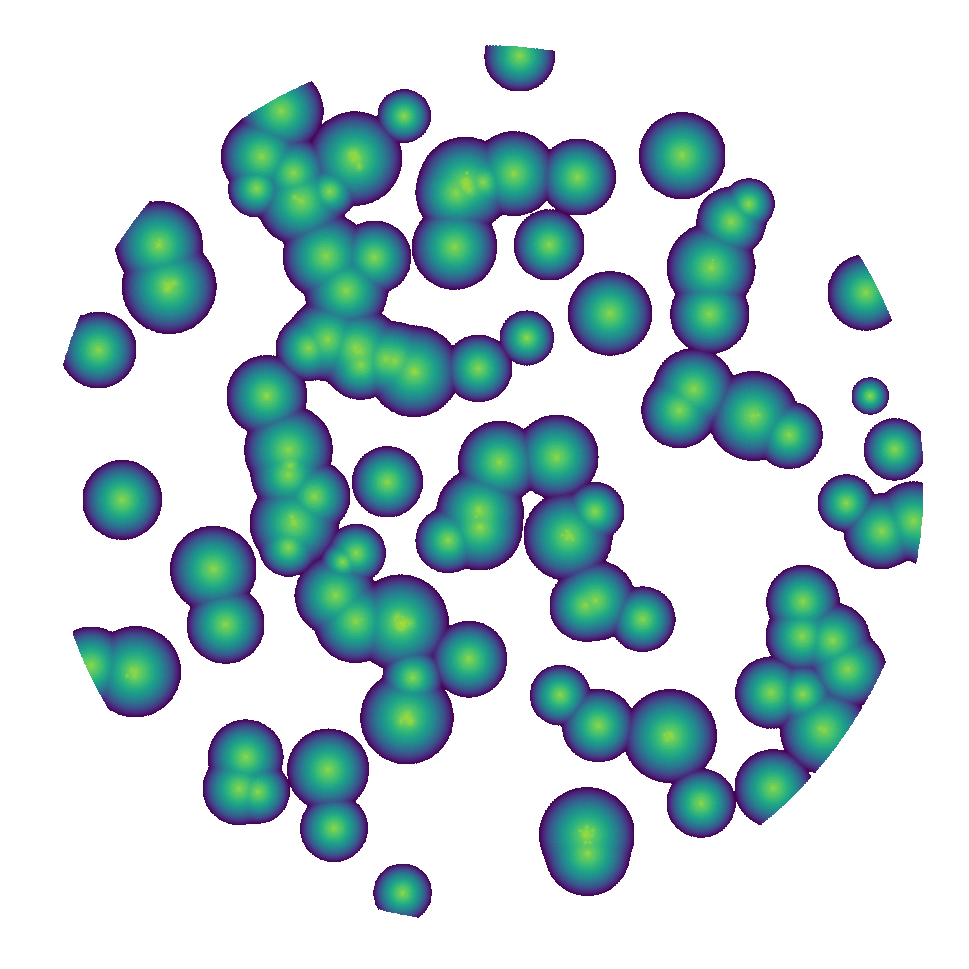
\includegraphics[width=0.48\textwidth]{Figures/Full-Dish-VirusPhotos/virus19.png}}

    \resizebox{0.48\textwidth}{!}{%
        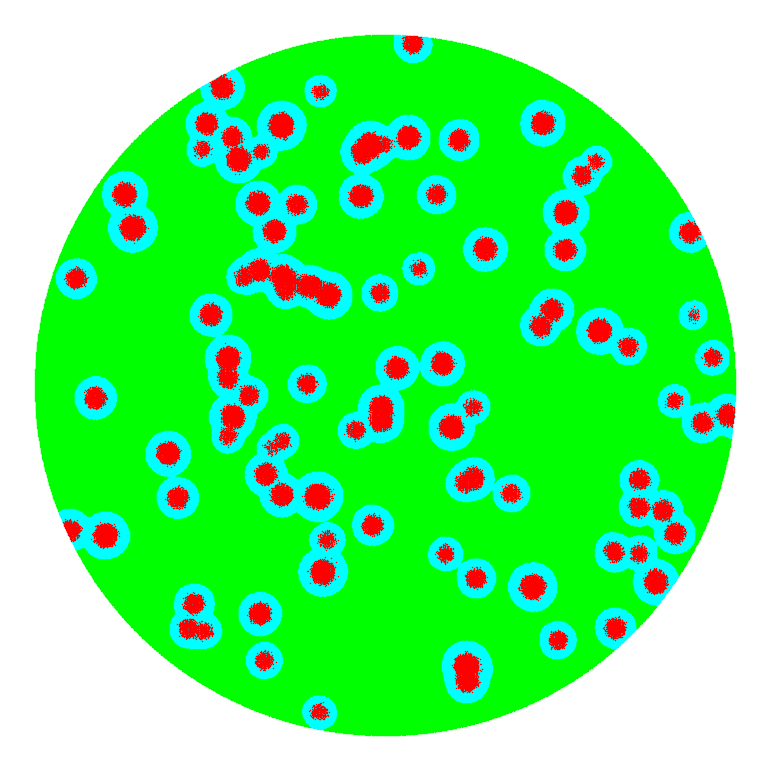
\includegraphics[width=0.48\textwidth]{Figures/Full-Dish-CellPhotos/cell29.png}
        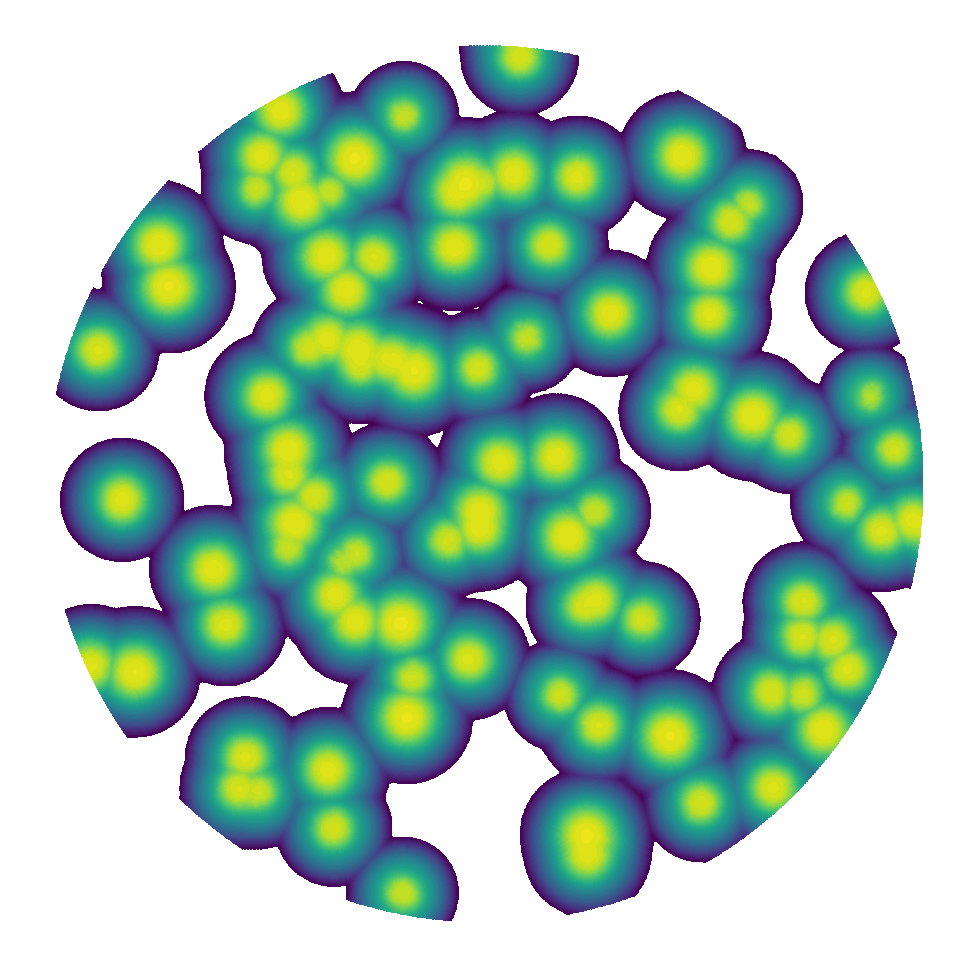
\includegraphics[width=0.48\textwidth]{Figures/Full-Dish-VirusPhotos/virus29.png}}

    \resizebox{0.48\textwidth}{!}{%
        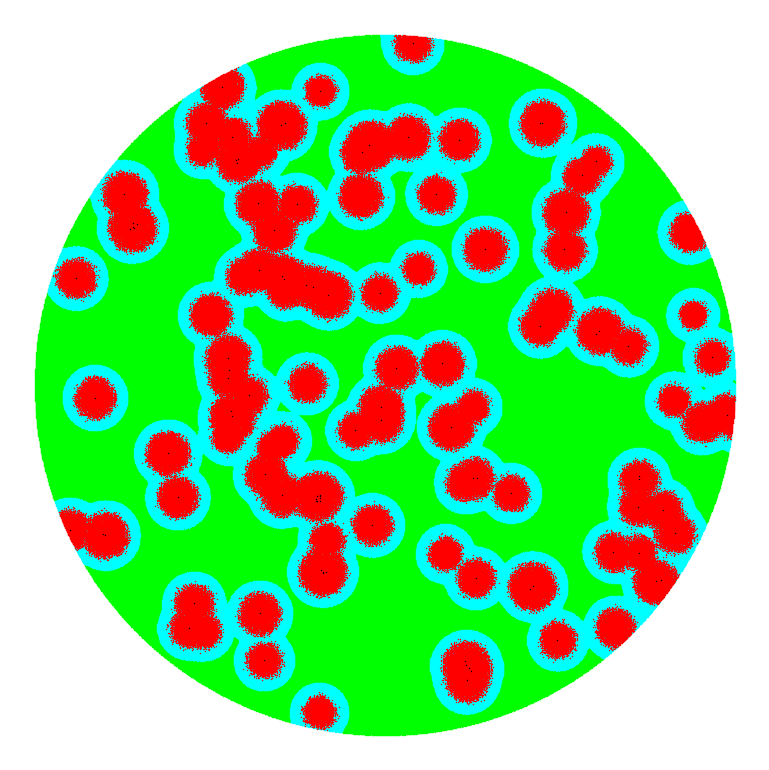
\includegraphics[width=0.48\textwidth]{Figures/Full-Dish-CellPhotos/cell39.png}
        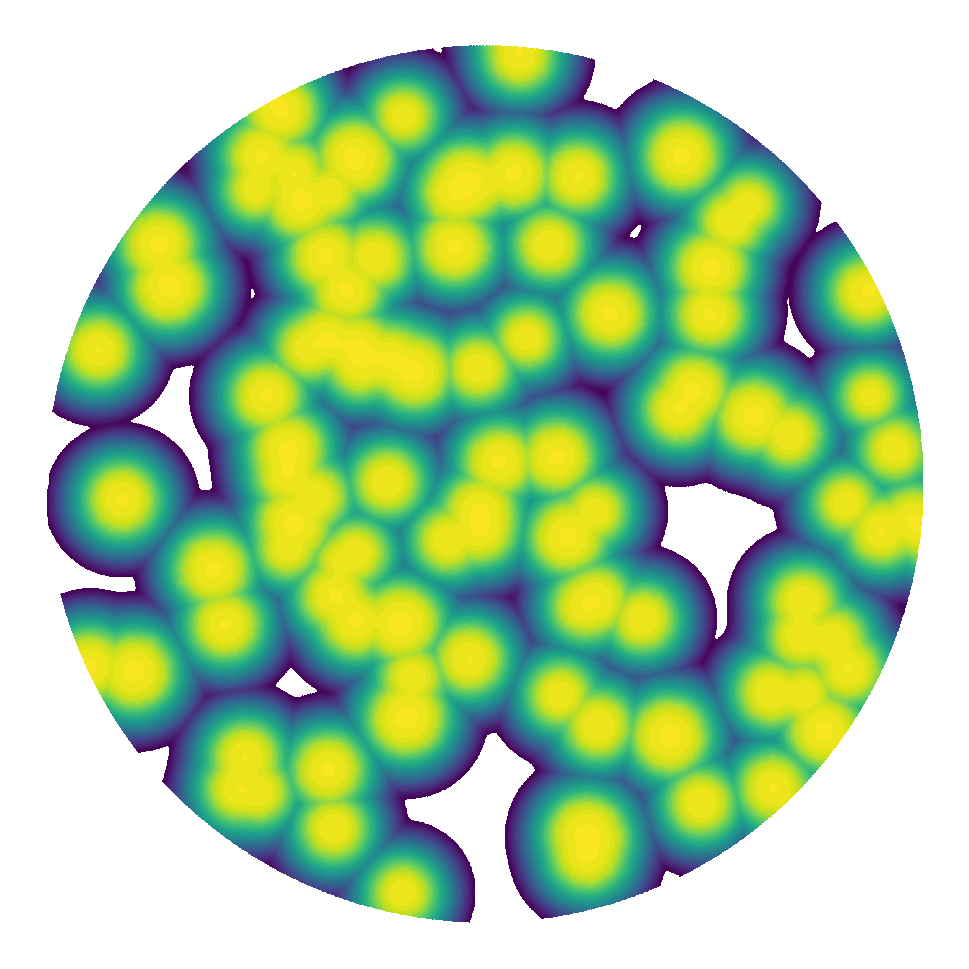
\includegraphics[width=0.48\textwidth]{Figures/Full-Dish-VirusPhotos/virus39.png}}

    \resizebox{0.48\textwidth}{!}{%
        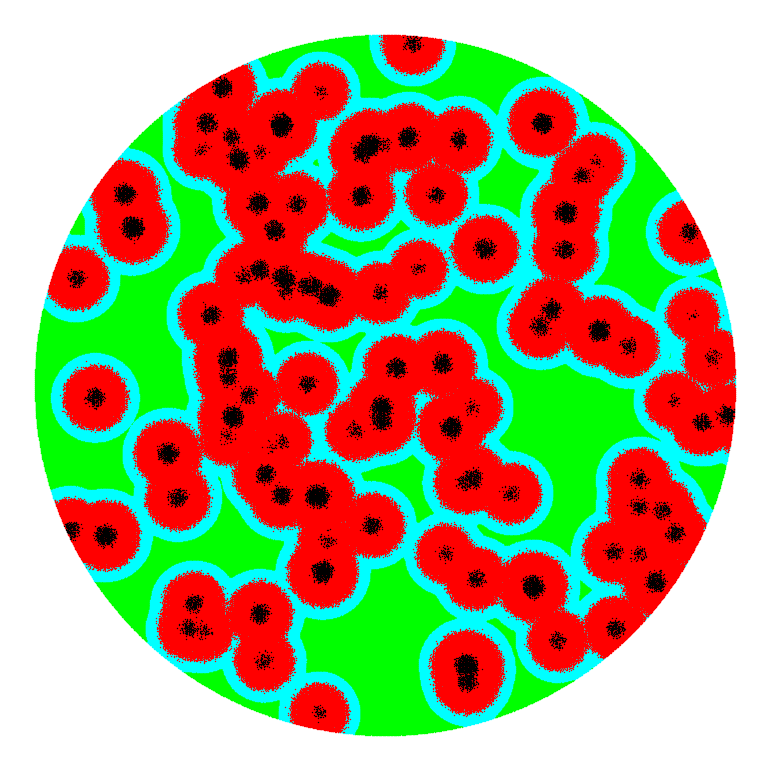
\includegraphics[width=0.48\textwidth]{Figures/Full-Dish-CellPhotos/cell49.png}
        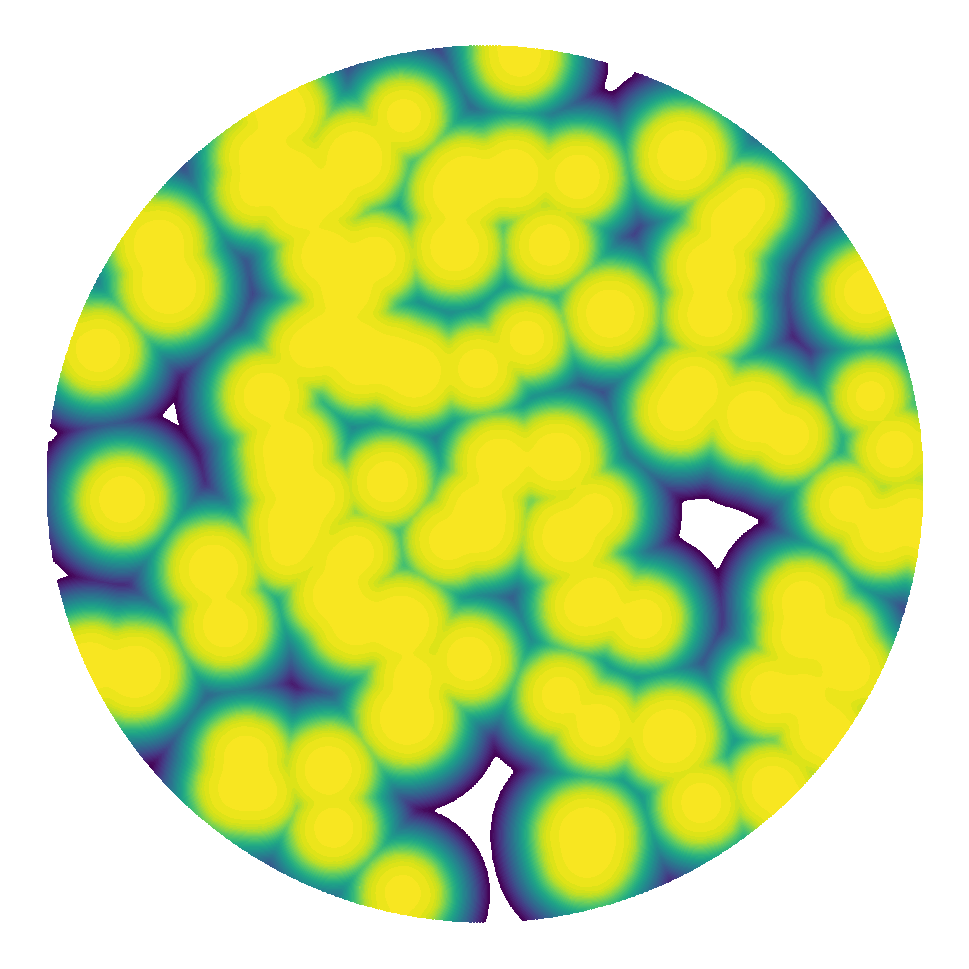
\includegraphics[width=0.48\textwidth]{Figures/Full-Dish-VirusPhotos/virus49.png}}

    \resizebox{0.48\textwidth}{!}{%
        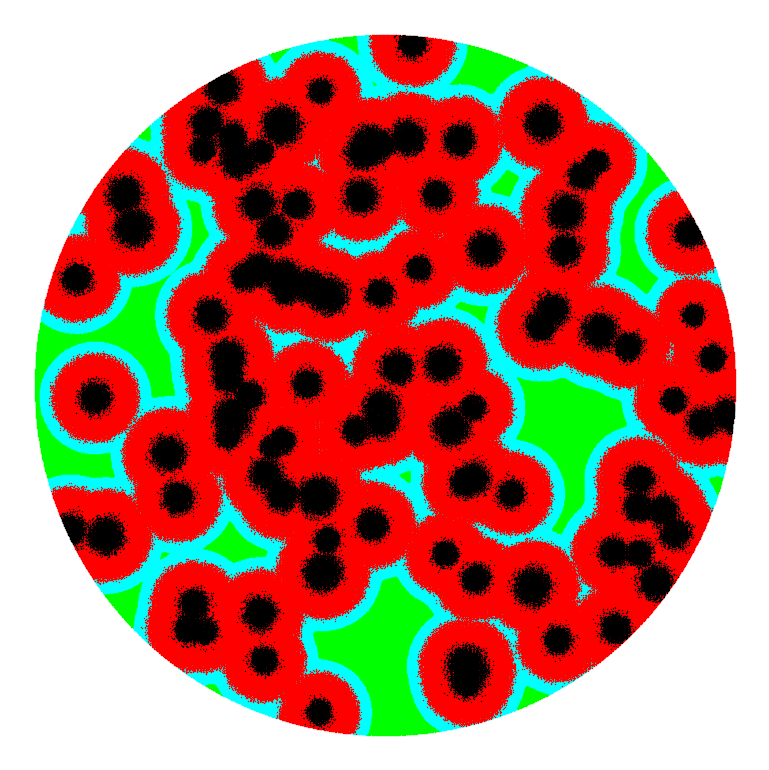
\includegraphics[width=0.48\textwidth]{Figures/Full-Dish-CellPhotos/cell59.png}
        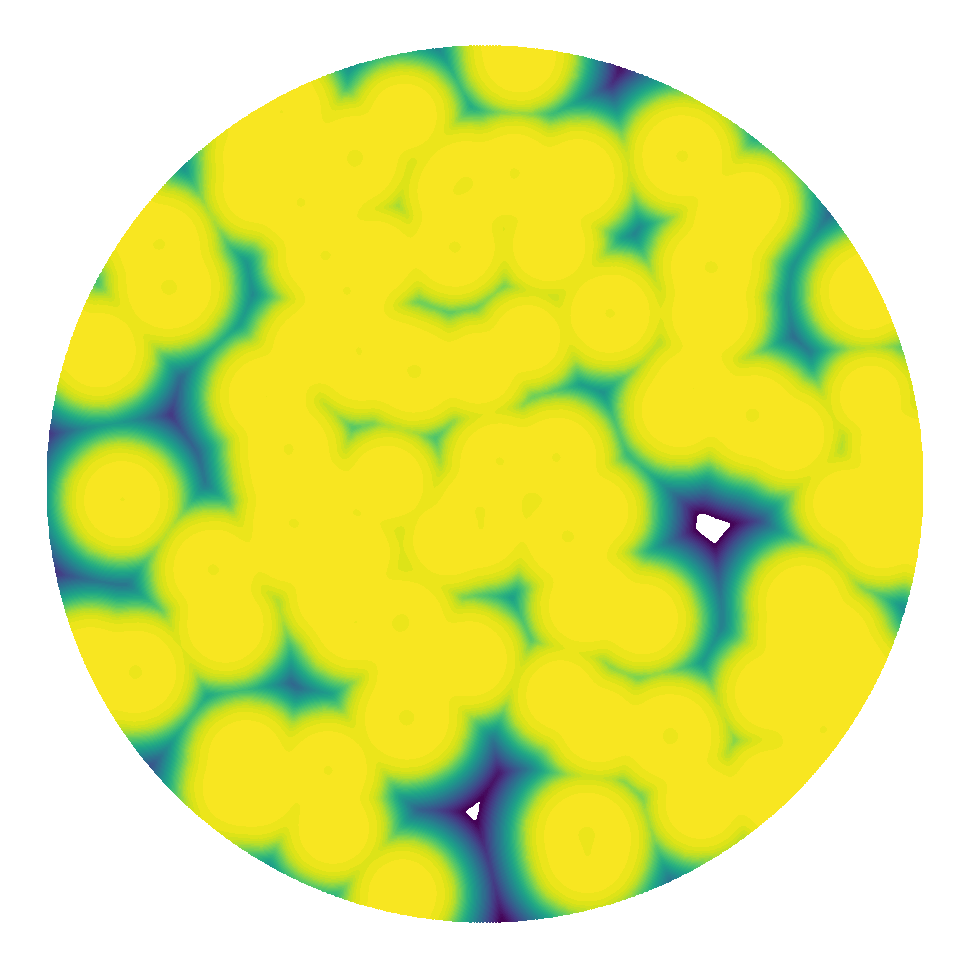
\includegraphics[width=0.48\textwidth]{Figures/Full-Dish-VirusPhotos/virus59.png}}

    \resizebox{0.48\textwidth}{!}{%
        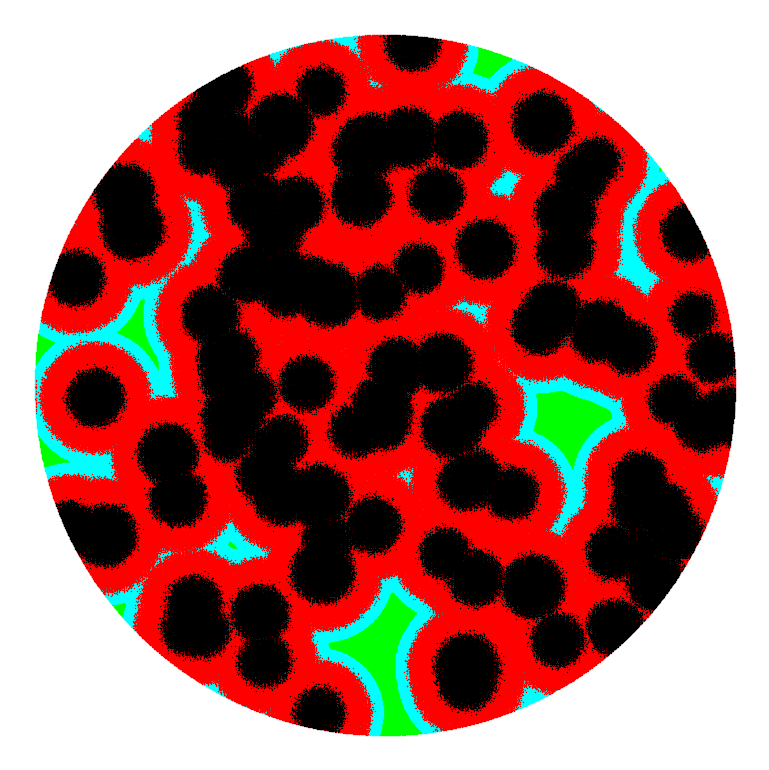
\includegraphics[width=0.48\textwidth]{Figures/Full-Dish-CellPhotos/cell69.png}
        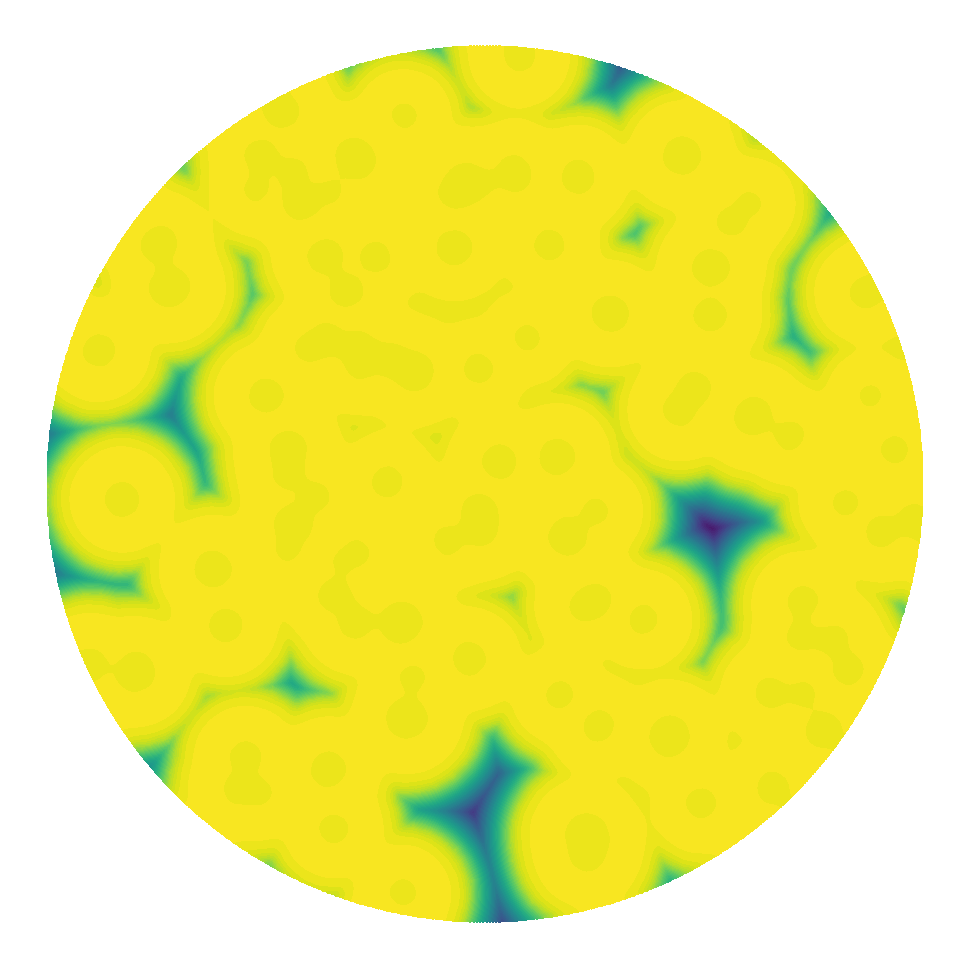
\includegraphics[width=0.48\textwidth]{Figures/Full-Dish-VirusPhotos/virus69.png}}

    \resizebox{0.48\textwidth}{!}{%
        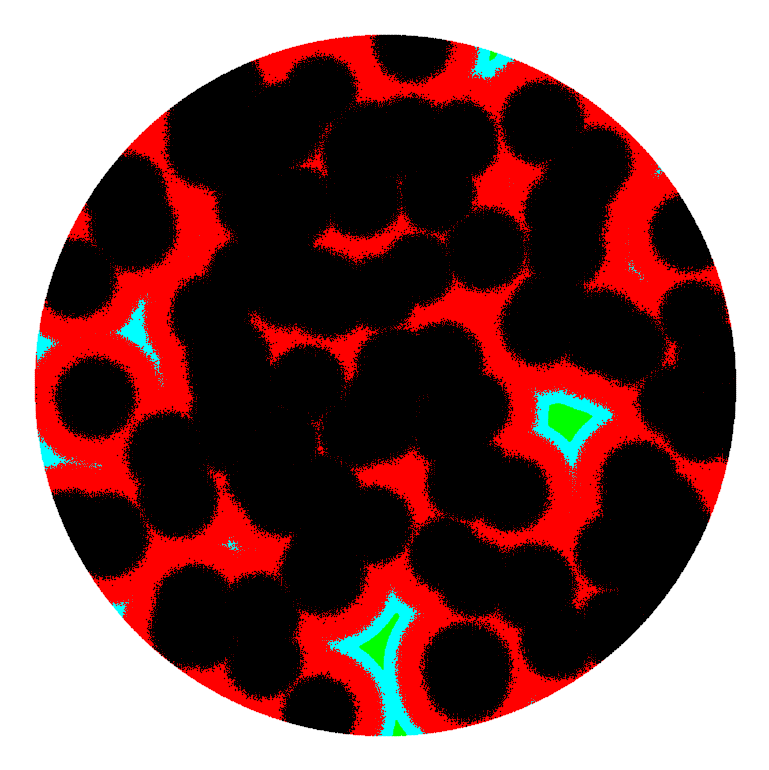
\includegraphics[width=0.48\textwidth]{Figures/Full-Dish-CellPhotos/cell79.png}
        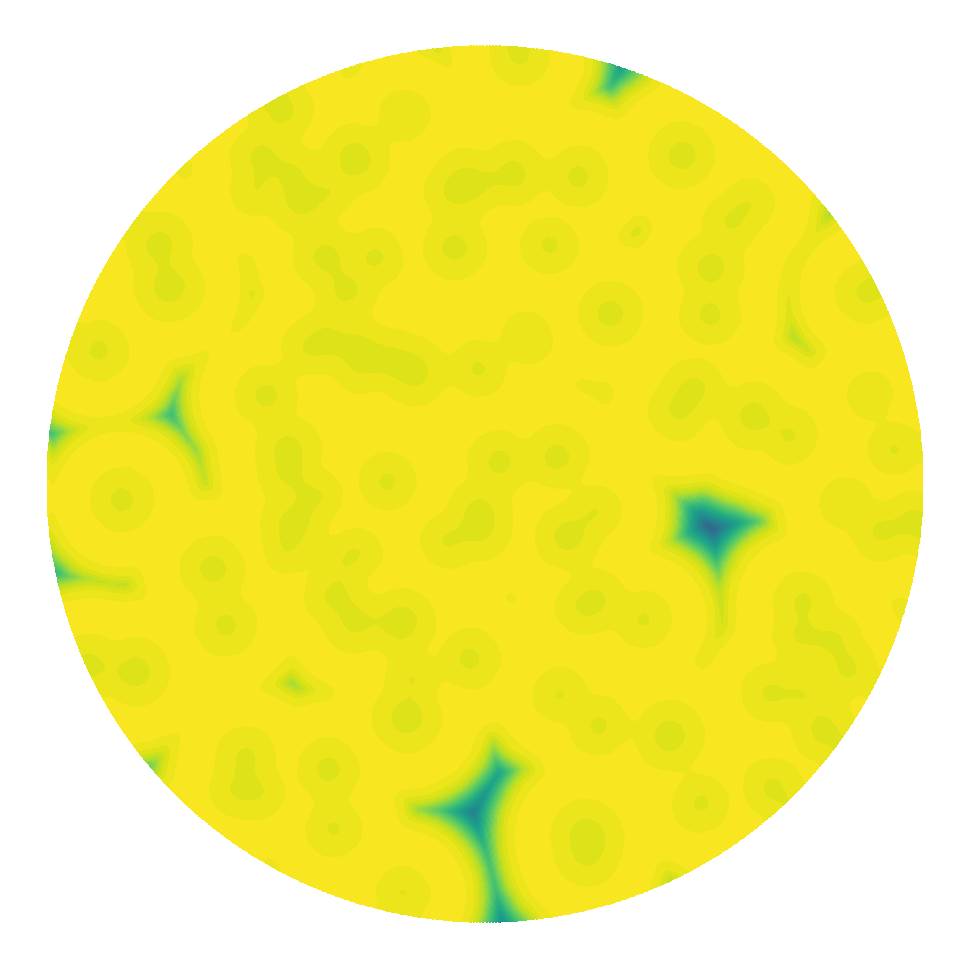
\includegraphics[width=0.48\textwidth]{Figures/Full-Dish-VirusPhotos/virus79.png}}

    \resizebox{0.48\textwidth}{!}{% 
        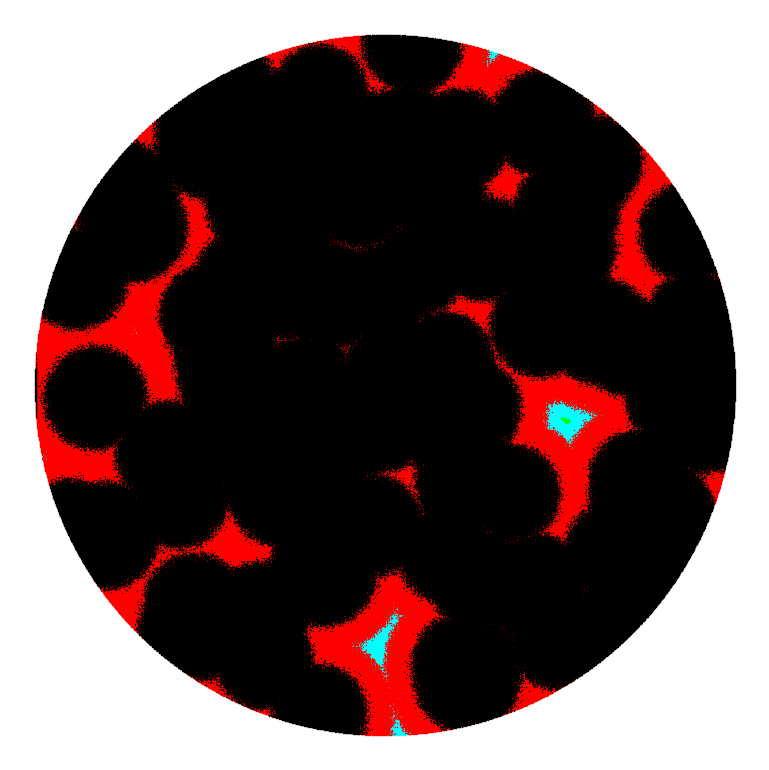
\includegraphics[width=0.48\textwidth]{Figures/Full-Dish-CellPhotos/cell89.png}
        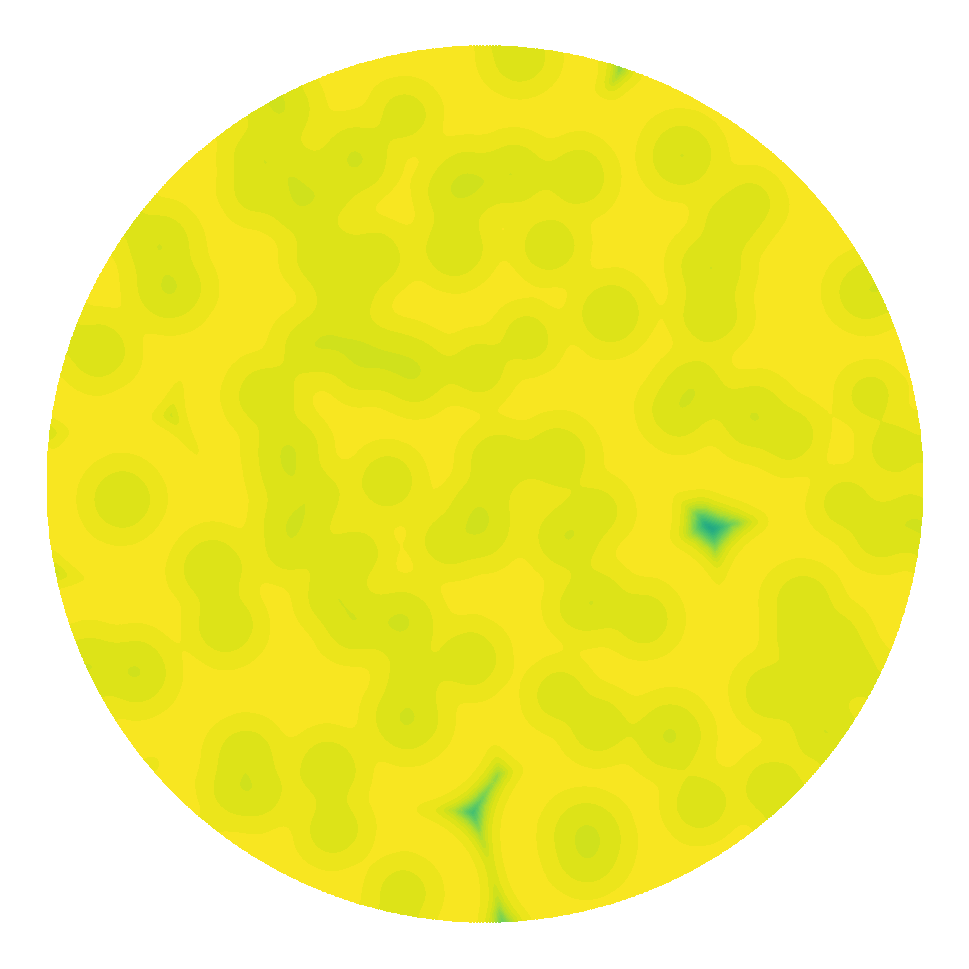
\includegraphics[width=0.48\textwidth]{Figures/Full-Dish-VirusPhotos/virus89.png}}

    \resizebox{0.48\textwidth}{!}{%
        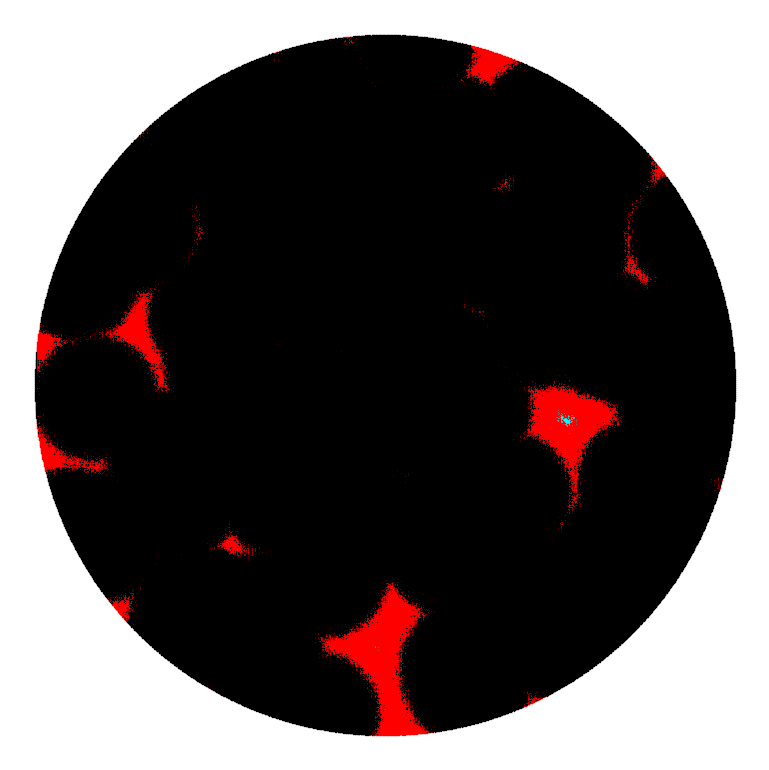
\includegraphics[width=0.48\textwidth]{Figures/Full-Dish-CellPhotos/cell99.png}
        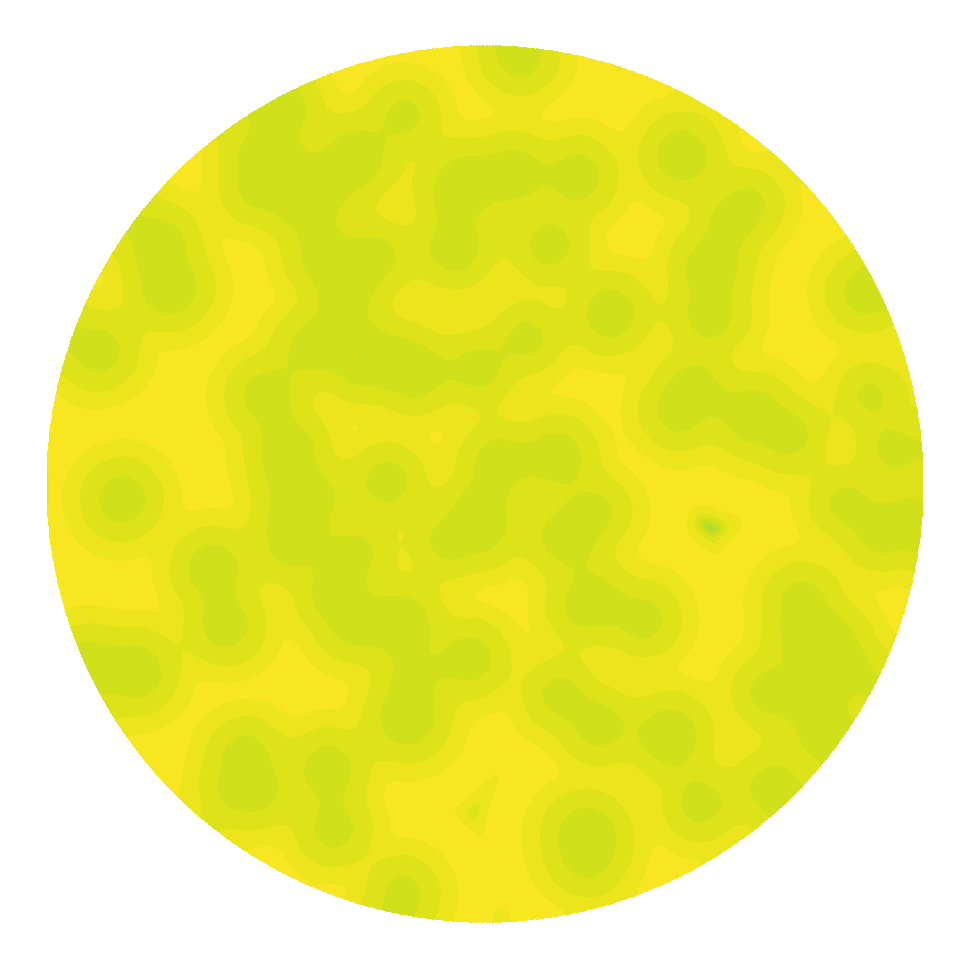
\includegraphics[width=0.48\textwidth]{Figures/Full-Dish-VirusPhotos/virus99.png}}

    \resizebox{0.48\textwidth}{!}{%
        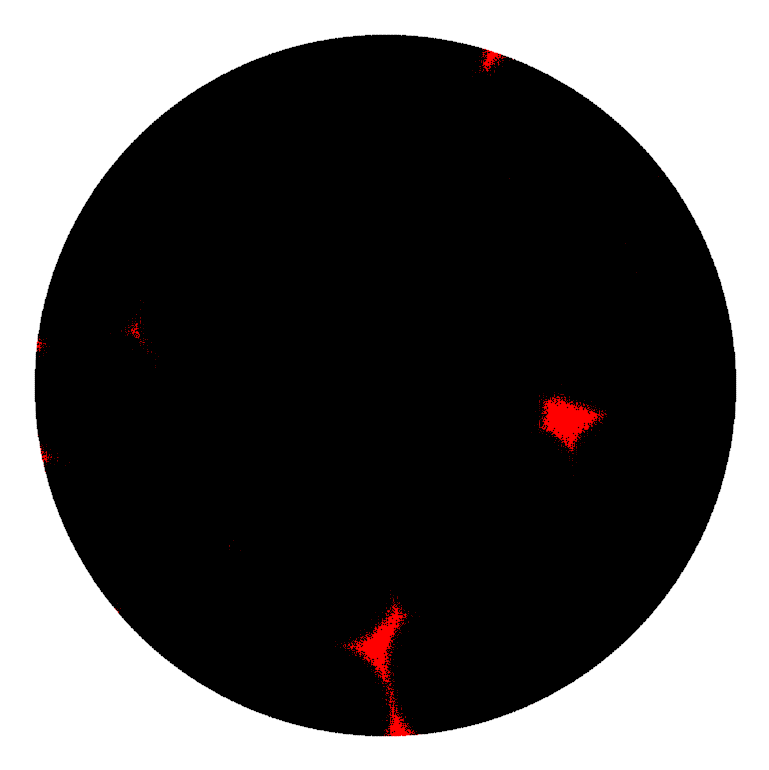
\includegraphics[width=0.48\textwidth]{Figures/Full-Dish-CellPhotos/cell109.png}
        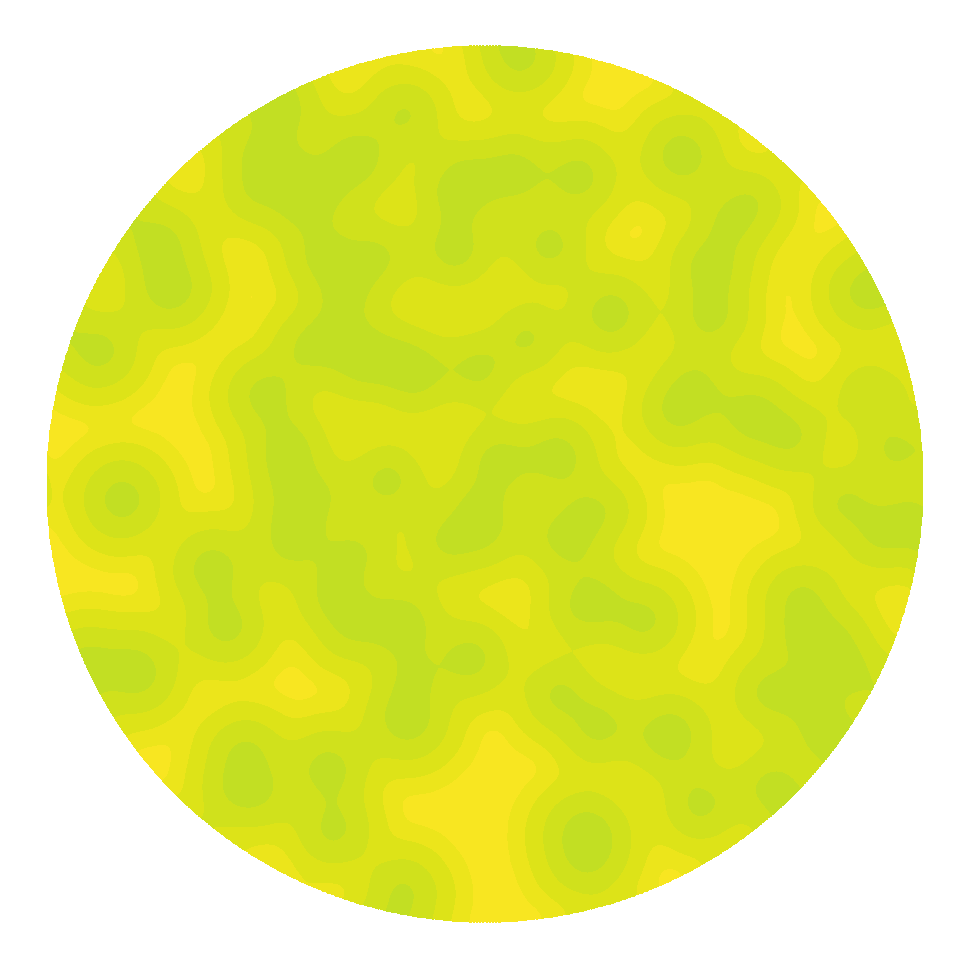
\includegraphics[width=0.48\textwidth]{Figures/Full-Dish-VirusPhotos/virus109.png}}

    \resizebox{0.48\textwidth}{!}{%
        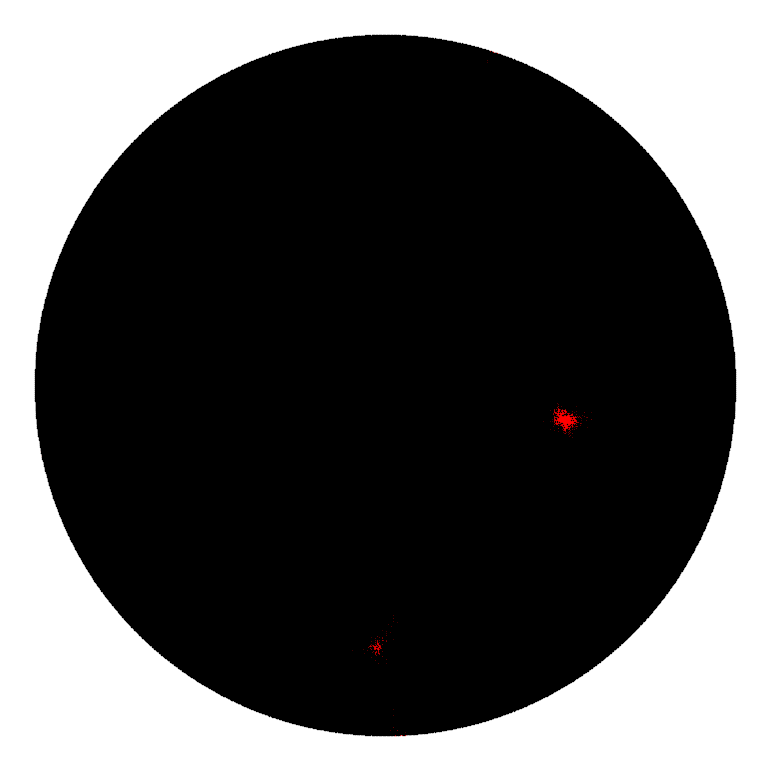
\includegraphics[width=0.48\textwidth]{Figures/Full-Dish-CellPhotos/cell119.png}
        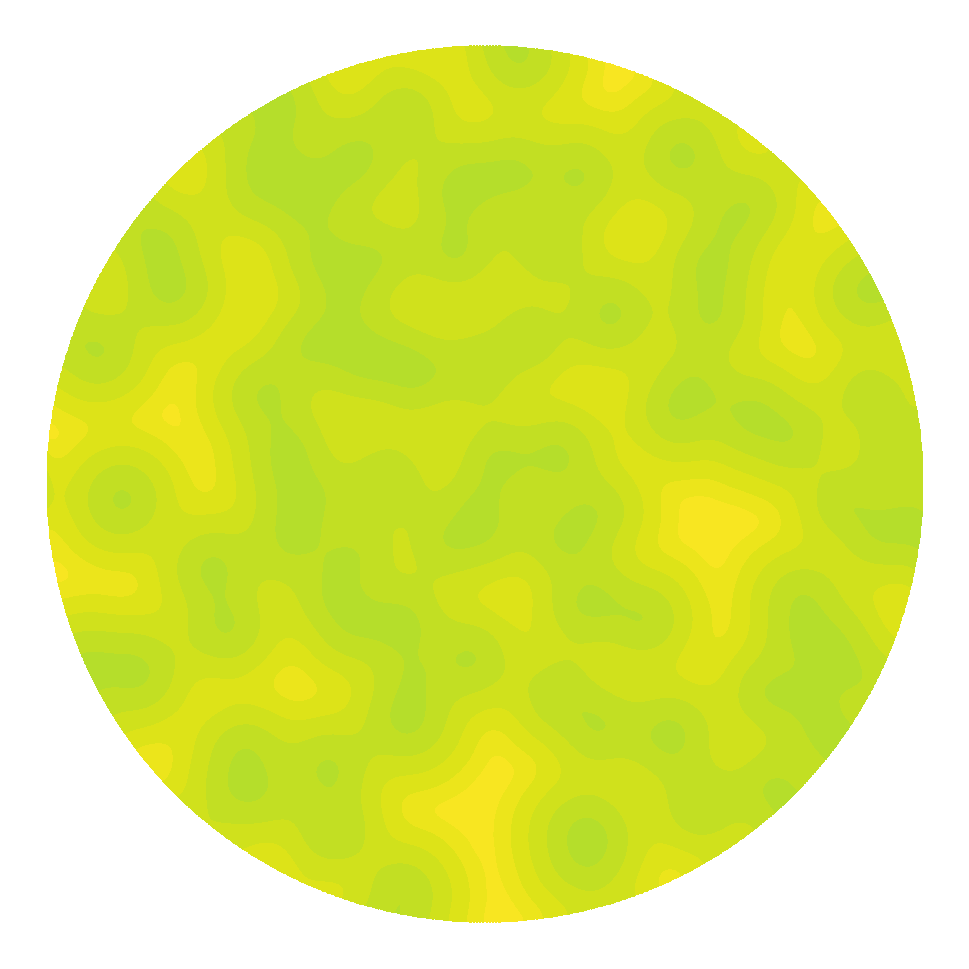
\includegraphics[width=0.48\textwidth]{Figures/Full-Dish-VirusPhotos/virus119.png}}

\end{multicols}
\end{minipage}
\caption{The dish at hours 5 through 60 in 5 hour increments. On the left are cells in the different stages of infection; the stages are represented by healthy cells colored green, eclipse cells colored cyan, infected cells colored red, and dead cells colored black. On the right are images of the virions that are diffusing over the cells; areas of higher concentration are represented by yellow and areas of lower concentration are represented by purple. \label{fig_FullDish_cellandvirus}}
\end{figure}

\begin{figure}
\centering
\begin{minipage}{0.66\linewidth}
\centering
    \resizebox{\textwidth}{!}{%
        
\includegraphics[width=0.48\textwidth]{Figures/Zoomed-In-CellPhotos/cell12.png}
        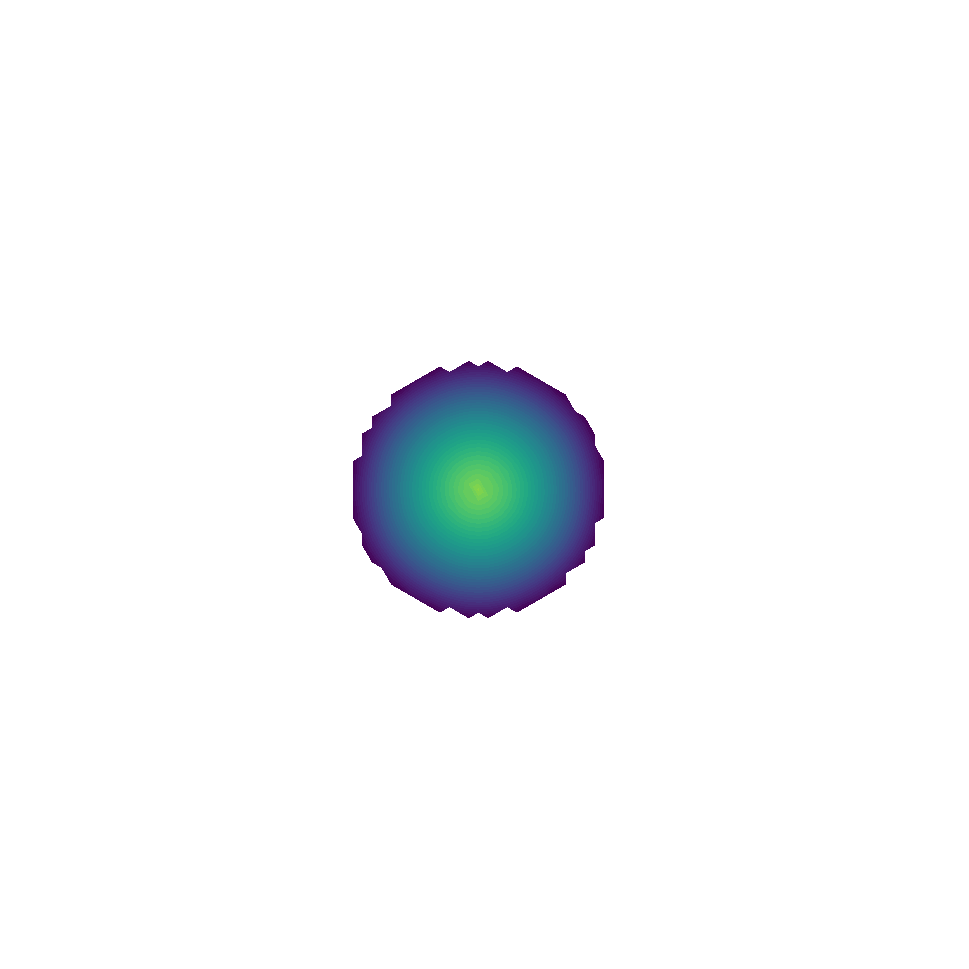
\includegraphics[width=0.48\textwidth]{Figures/Zoomed-In-VirusPhotos/virus12.png}}

    \vspace{0.25em}
    \resizebox{\textwidth}{!}{%
        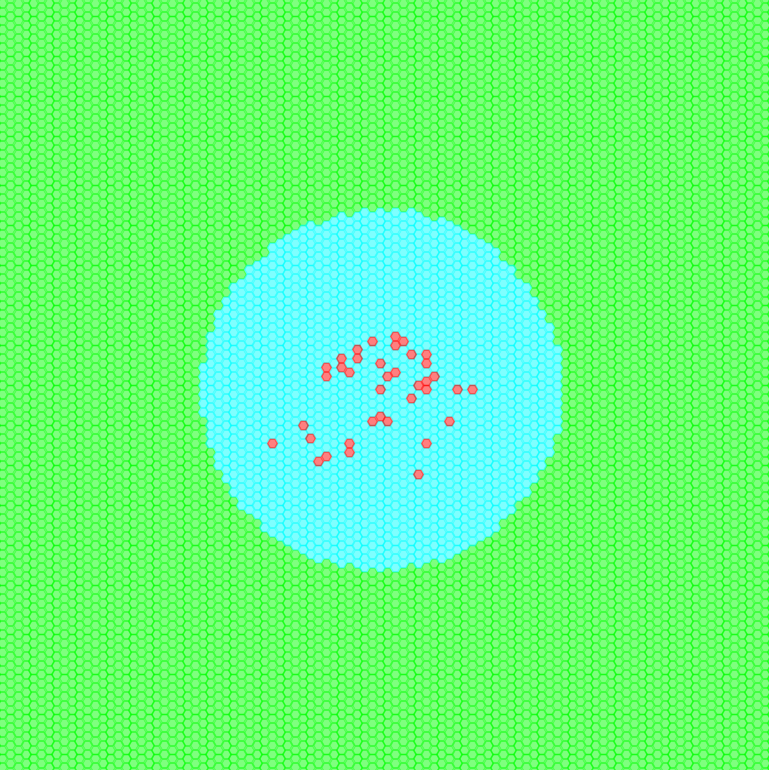
\includegraphics[width=0.48\textwidth]{Figures/Zoomed-In-CellPhotos/cell22.png}
        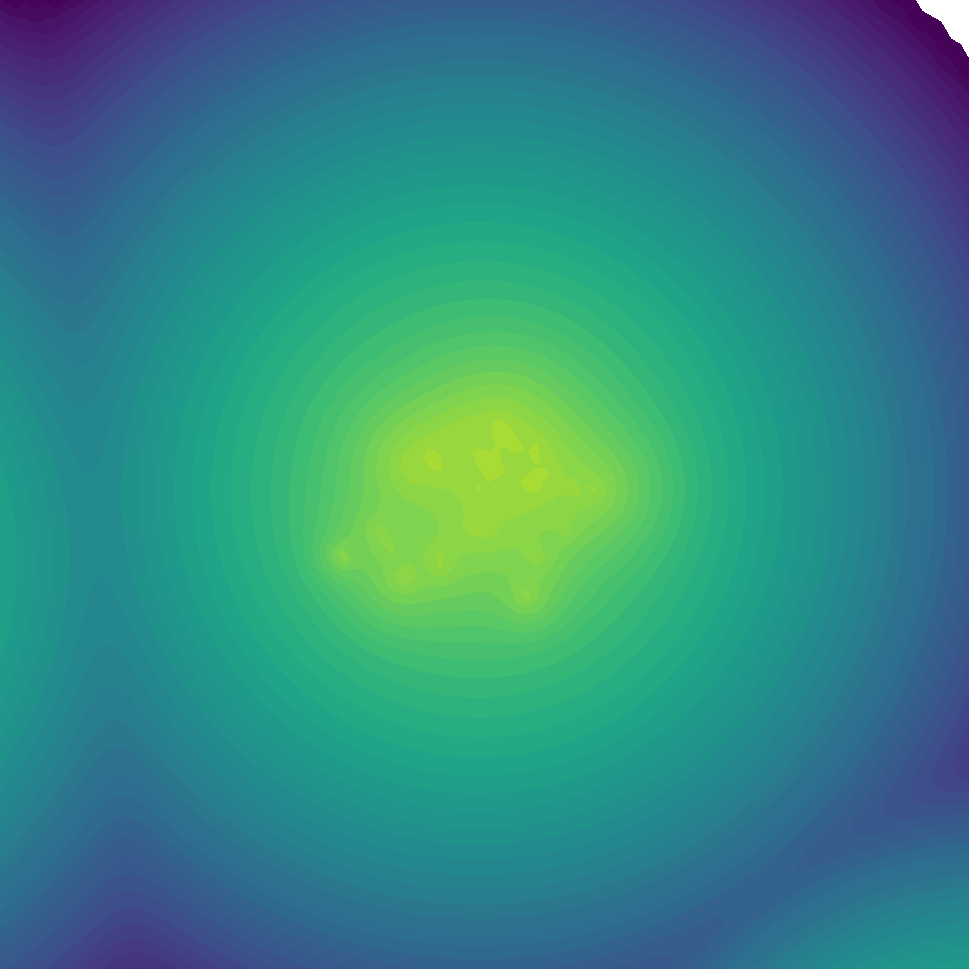
\includegraphics[width=0.48\textwidth]{Figures/Zoomed-In-VirusPhotos/virus22.png}}

    \vspace{0.25em}
    \resizebox{\textwidth}{!}{%
        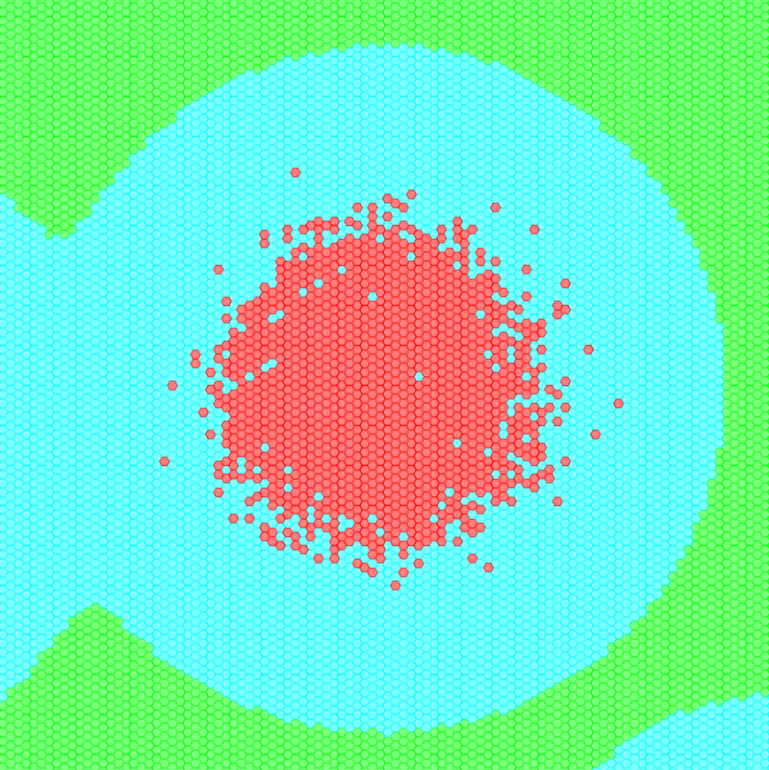
\includegraphics[width=0.48\textwidth]{Figures/Zoomed-In-CellPhotos/cell32.png}
        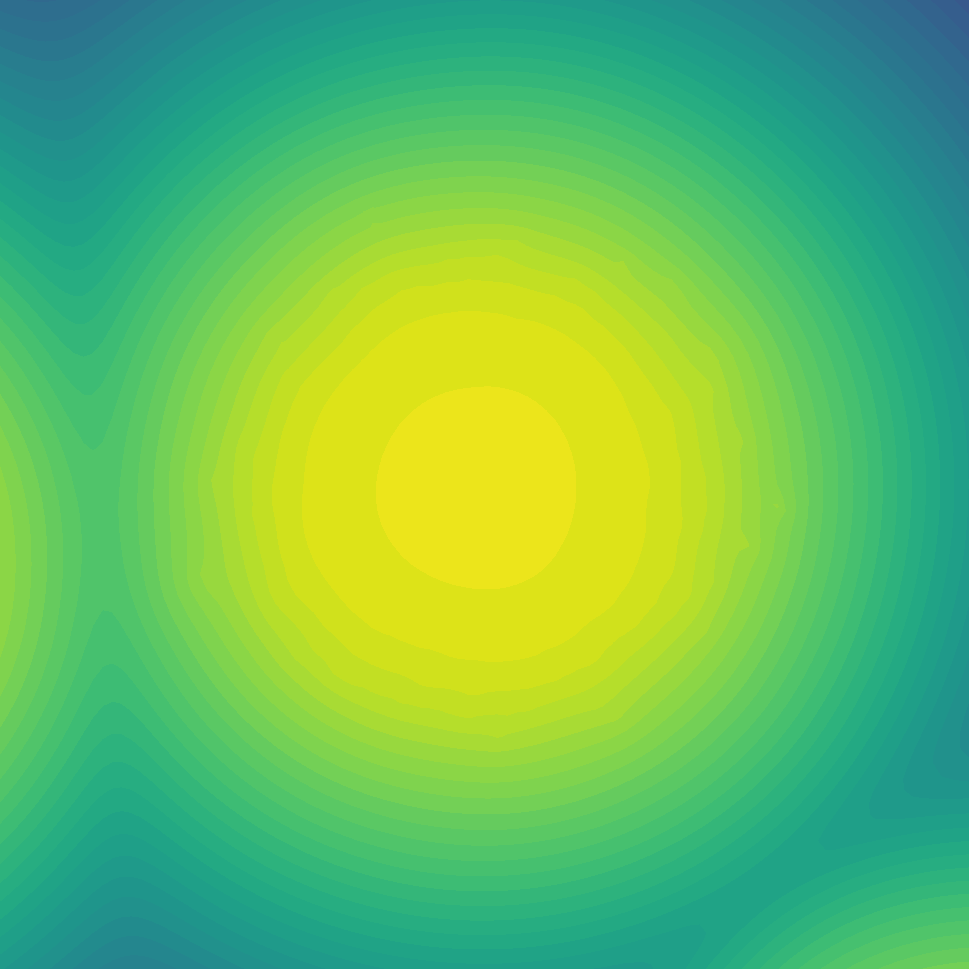
\includegraphics[width=0.48\textwidth]{Figures/Zoomed-In-VirusPhotos/virus32.png}}
\end{minipage}
\caption{A zoomed in section of the dish looking at the plaque formed by a single infected cell during a viral infection at hours 6.5, 11.5, and 16.5. On the left are cells in the different stages of infection; the stages are represented by healthy cells colored green, eclipse cells colored cyan, infected cells colored red, and dead cells colored black. On the right are the many virus that are diffusing over the cells; areas of higher concentration are represented by yellow and areas of lower concentration are represented by purple. \label{fig_ZoominDish}}
\end{figure}


%\begin{figure}
%\captionsetup[subfigure]{aboveskip=-1pt,belowskip=1pt}
%\centering
%\parbox{0.66\textwidth}{%
%    \hspace{-0.6875em}
%    \resizebox{0.33\textwidth}{!}{
\includegraphics{Figures/Zoomed-In-CellPhotos/cell12.png}}
%    \resizebox{0.33\textwidth}{!}{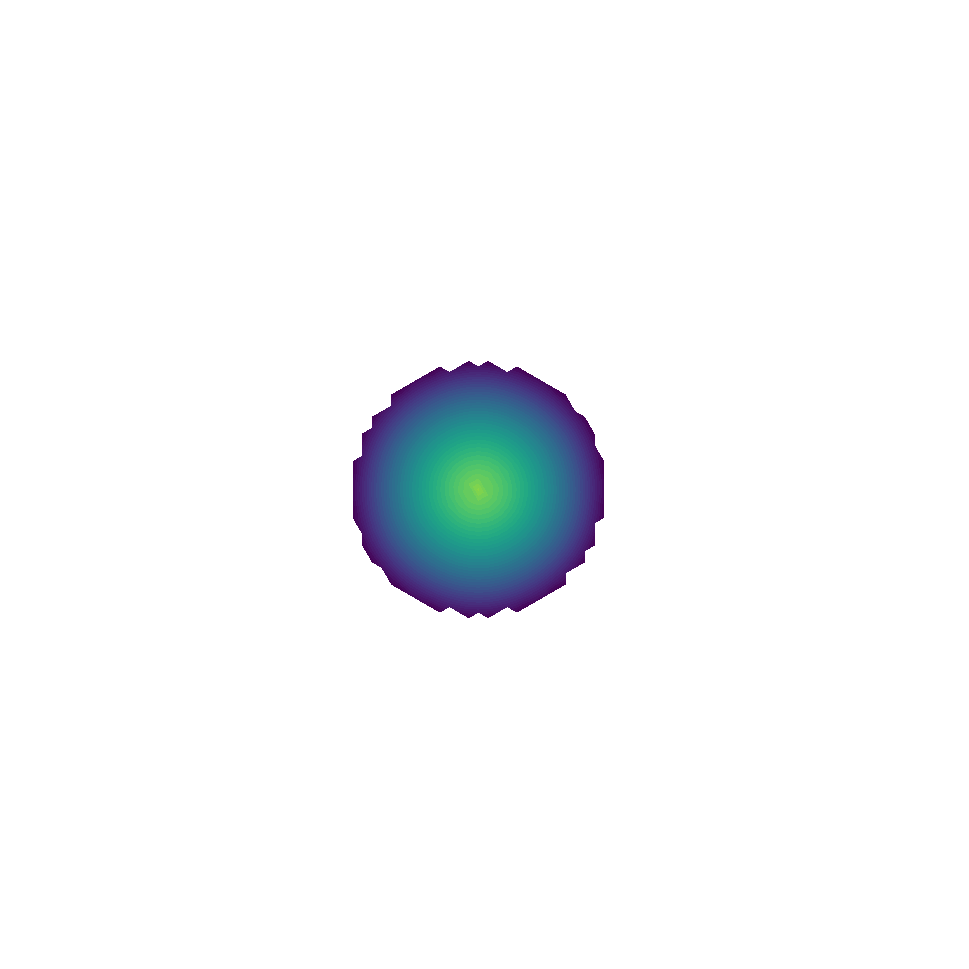
\includegraphics{Figures/Zoomed-In-VirusPhotos/virus12.png}}

%    \vspace{0.25em}
%    \hspace{-0.6875em}
%    \resizebox{0.33\textwidth}{!}{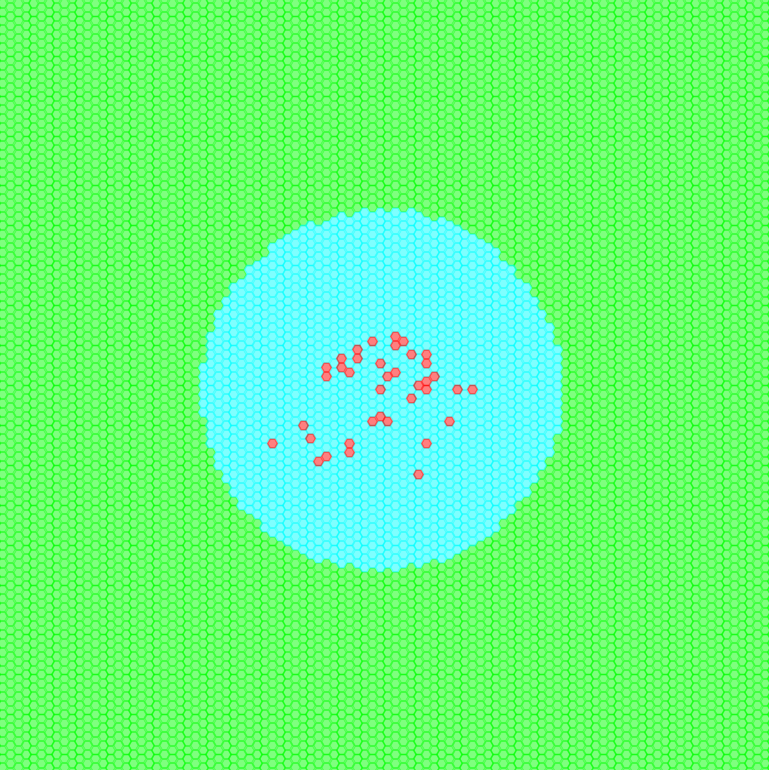
\includegraphics{Figures/Zoomed-In-CellPhotos/cell22.png}}
%    \resizebox{0.33\textwidth}{!}{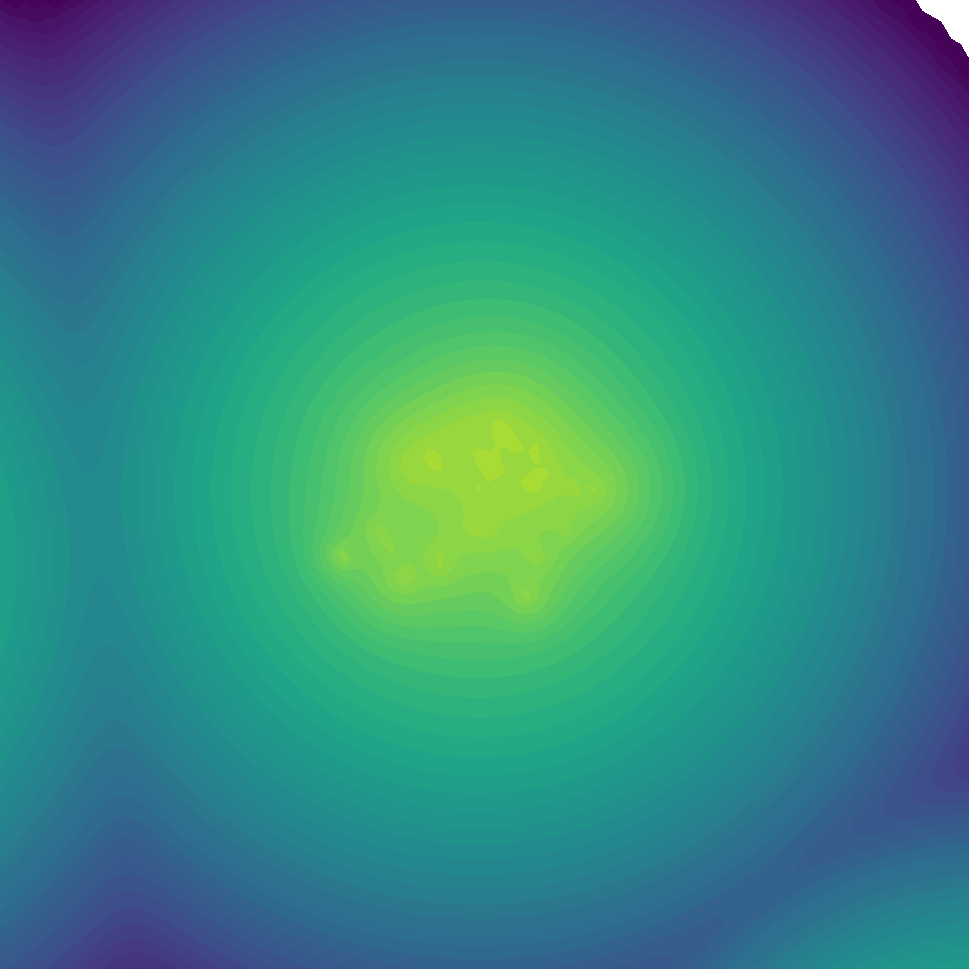
\includegraphics{Figures/Zoomed-In-VirusPhotos/virus22.png}}

%    \vspace{0.25em}
%    \hspace{-0.6875em}
%    \resizebox{0.33\textwidth}{!}{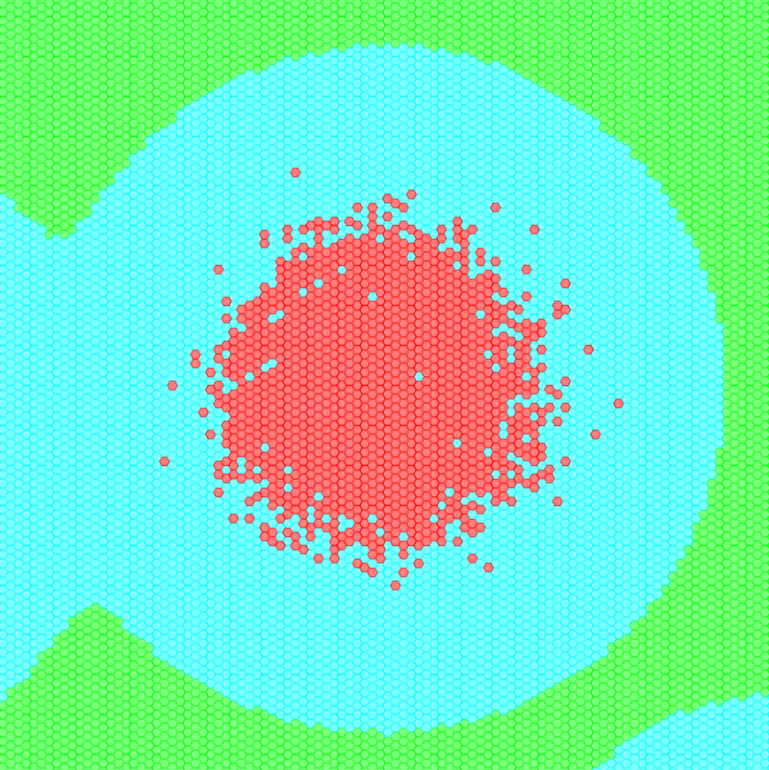
\includegraphics{Figures/Zoomed-In-CellPhotos/cell32.png}}
%    \resizebox{0.33\textwidth}{!}{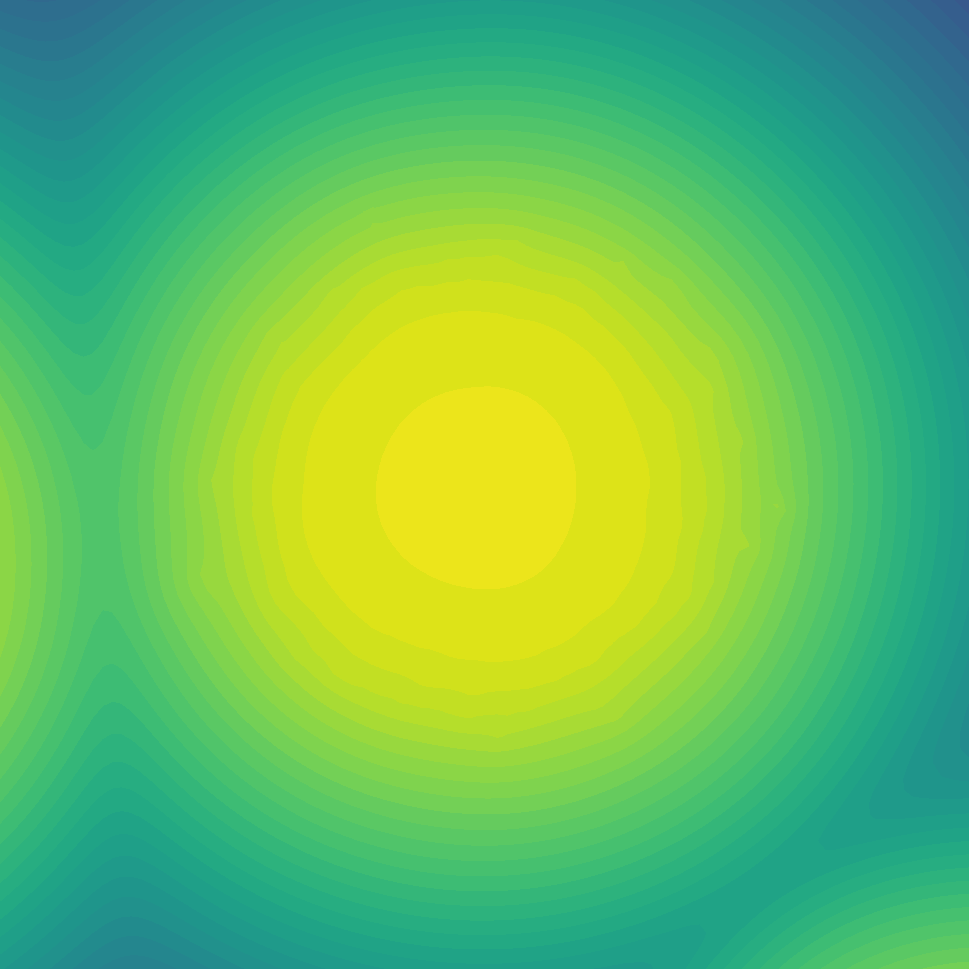
\includegraphics{Figures/Zoomed-In-VirusPhotos/virus32.png}}}

%    \caption{A zoomed in section of the dish looking at the plaque formed by a single infected cell during a viral infection at hours 6.5, 11.5, and 16.5. On the left are cells in the different stages of infection; the stages are represented by healthy cells colored green, eclipse cells colored cyan, infected cells colored red, and dead cells colored black. On the right are the many virus that are diffusing over the cells; areas of higher concentration are represented by yellow and areas of lower concentration are represented by purple. \label{fig_ZoominDish}}
%\end{figure}

%\clearpage
\subsection{Implementation on GPUs}

We simulated ten viral infections for five different numbers of cells, with codes that utilize three different programming languages: Python, C, and CUDA. The amount of computation time needed to simulate one hour of the infection, on a desktop computer, is shown in figure \ref{fig:SpeedComparison}. The computer was built with an Intel Xeon E-2144G CPU, 16 gigabytes of RAM, and P4000 Nvidia Graphics card. The compute times for the three codes increase as the number of cells in the simulations increases, but the speed increase of switching from Python, the programming language commonly used in physics, to code using CUDA for implementation on GPUs is 6954 times faster.
\begin{figure}
    \centering
    \resizebox{0.6\textwidth}{!}{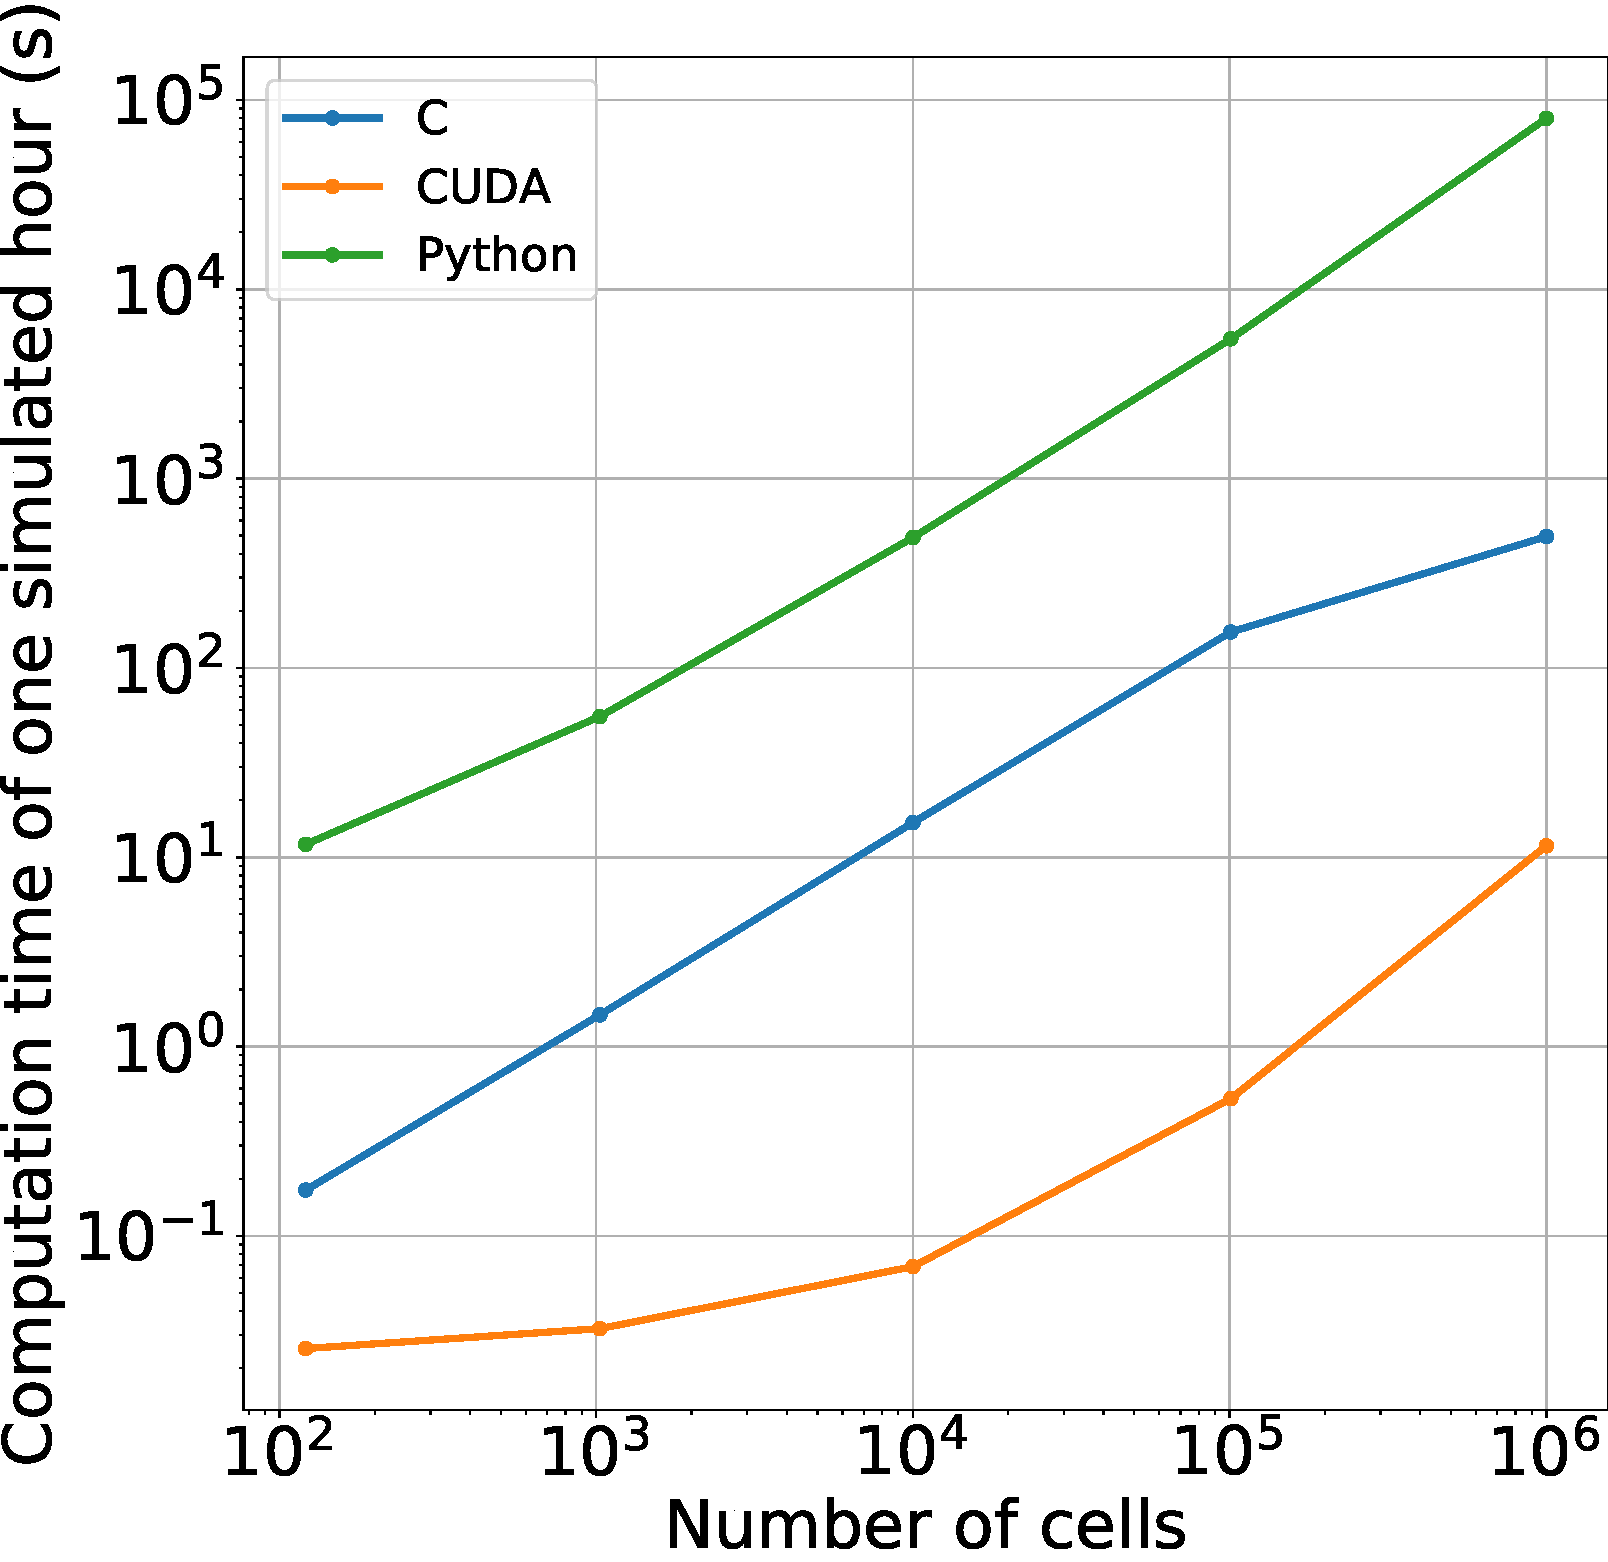
\includegraphics{Figures/loglogspeed.pdf}}
\caption{With more than a million cells, CUDA is 6954 times faster then the Python code and 43 time faster than the C code. \label{fig:SpeedComparison}}
\end{figure}

%\clearpage
\subsubsection{Convergence Testing}

We examine three scenarios when testing the convergence of the model: an infection initiated with $10013$ cells in the eclipse phase (Initial Cell); an infection initiated with $10^{12}$ virions (Initial Virus); and a scenario with no infection, but $10^{12}$ virions (Only Virus), examining viral spread and decay only. Simulations in each of the scenarios used the influenza parameters from Table \ref{tab_params}. Figure \ref{fig:ViralTiterCurves} shows the simulations of the three scenarios, where the time step was varied to test the convergence of the model in time. A time step of 0.005 hr was chosen and a range around it was made by dividing or multiplying by 2 repeatedly. This formed an array of seven time step values, 0.000625, 0.00128, 0.0025, 0.005, 0.01, 0.02, and 0.04 hr. For each time step, the median curve of ten viral titer curves is shown. In figure \ref{fig:ViralTiterCurves}, from left to right, curves of a viral infection initiated with infected cells; curves of a viral infection initiated with virus; and curves of virus without underlying cell infection. We see that for all the time steps, except $0.04$ hr, the curves are hard to distinguish from one another and follow the same trend for each scenario. 

\begin{figure}
    \centering
    \parbox{\textwidth}{
    \fbox{\parbox{\textwidth}{\vspace{-1em}
    \begin{multicols}{3}
        \centering

        Initial Cell

        Initial Virus

        Only Virus
    \end{multicols}
    \vspace{-1em}}}

    \vspace{0.5em}
    \centering
    \resizebox{0.32\textwidth}{!}{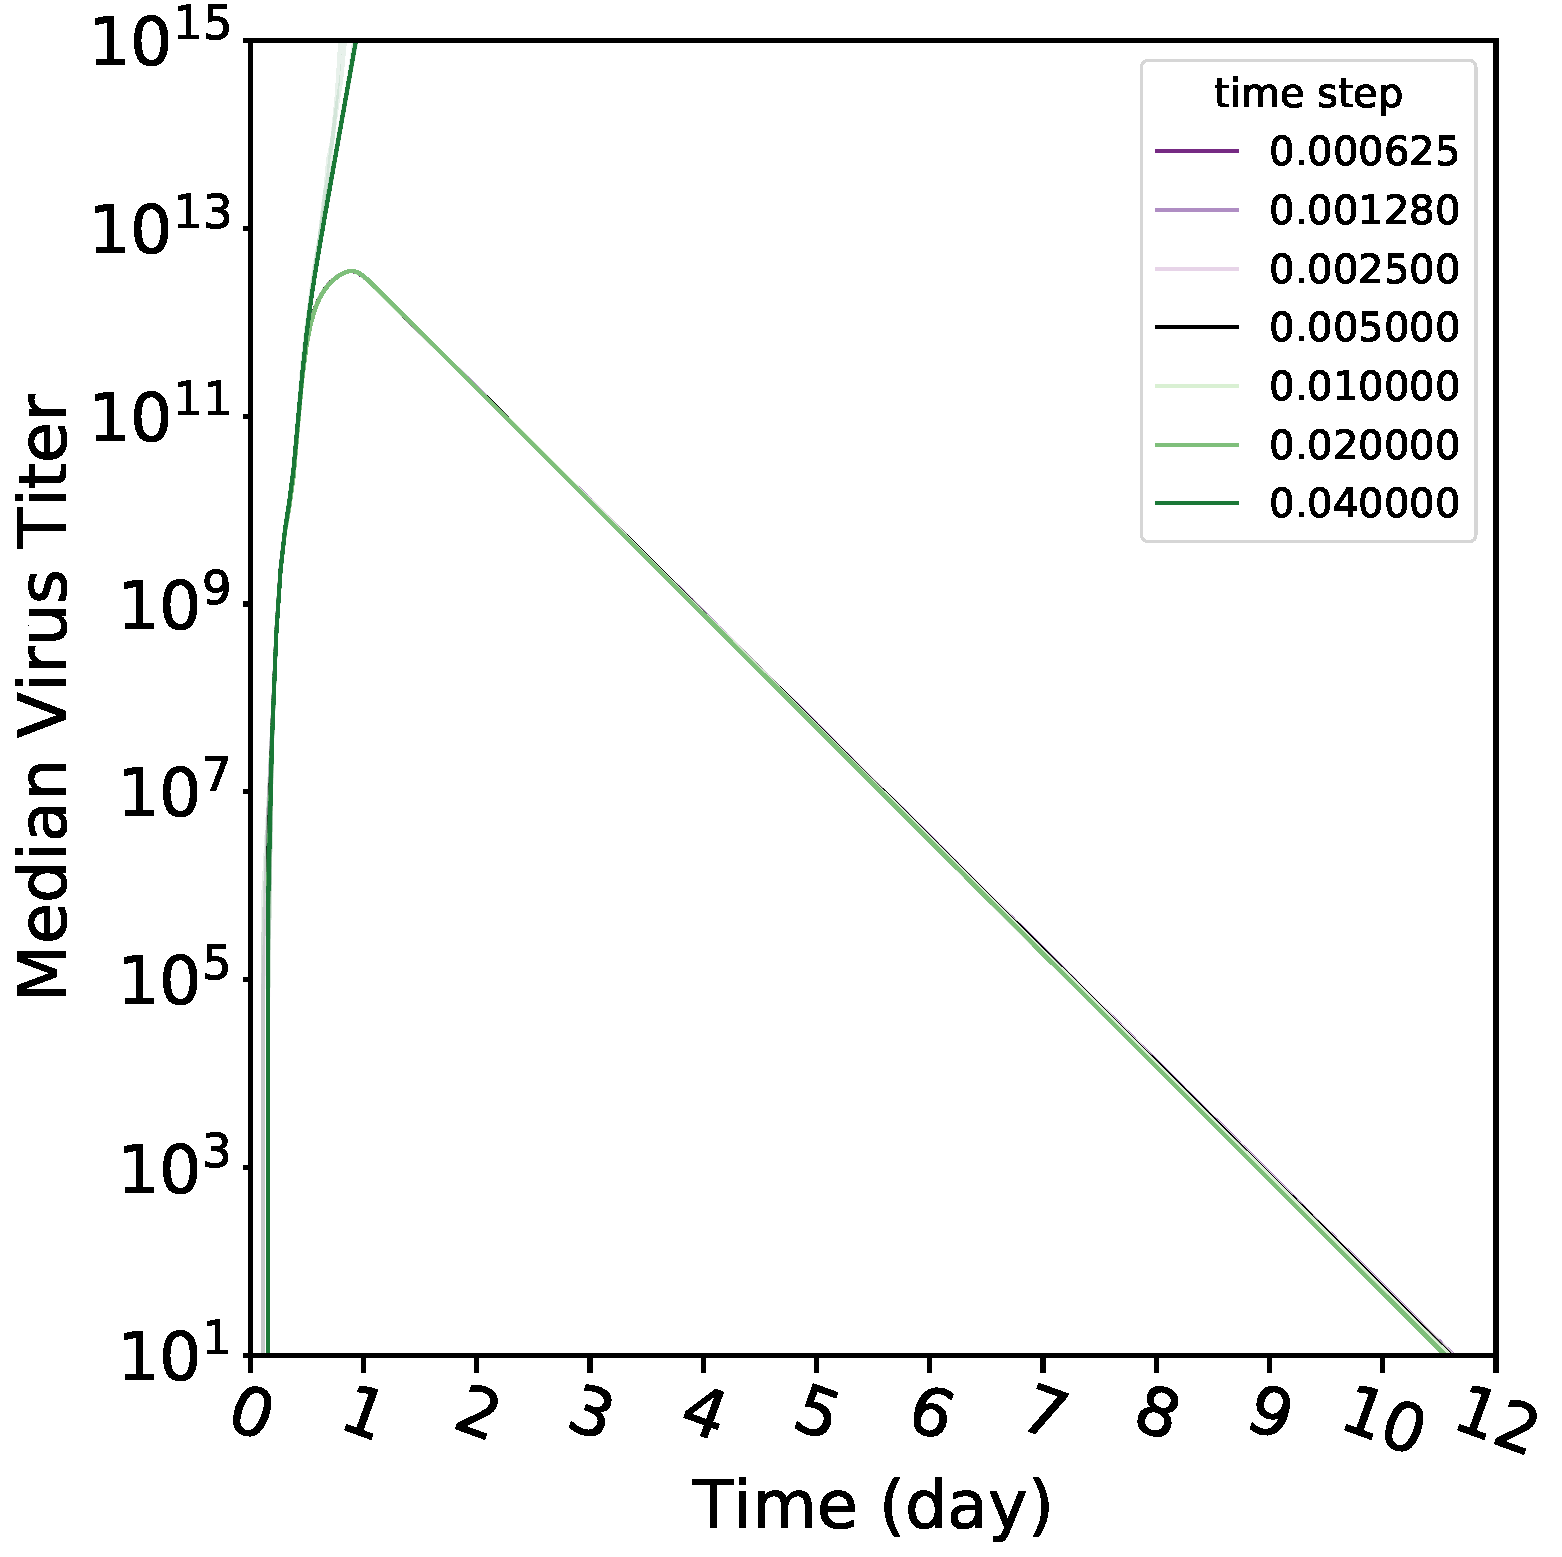
\includegraphics{Figures/Cellfree-InitialCell-AllOnOne_Median_VirusVsTime.pdf}}
    \resizebox{0.32\textwidth}{!}{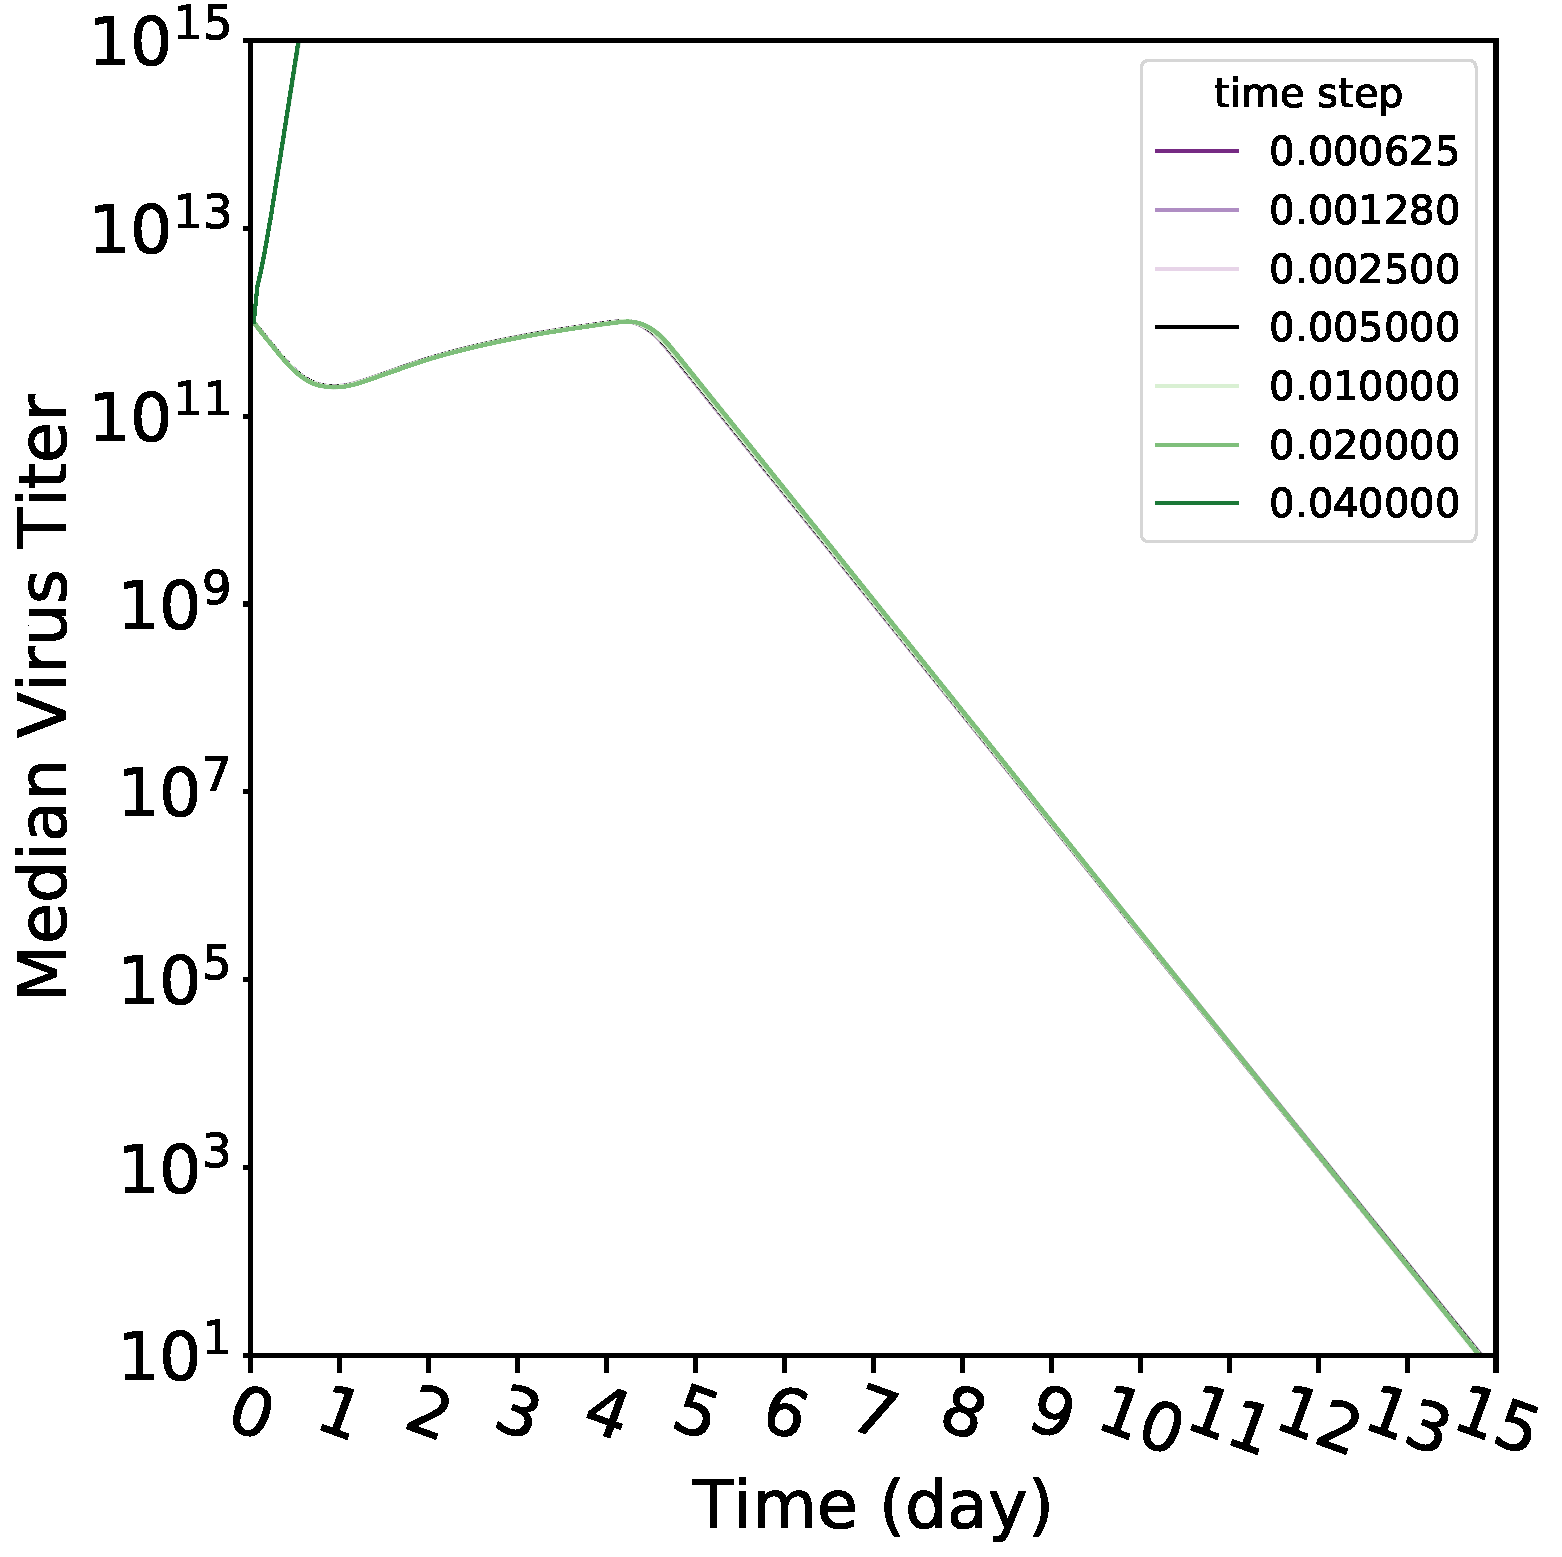
\includegraphics{Figures/Cellfree-InitialVirus-AllOnOne_Median_VirusVsTime.pdf}}
    \resizebox{0.32\textwidth}{!}{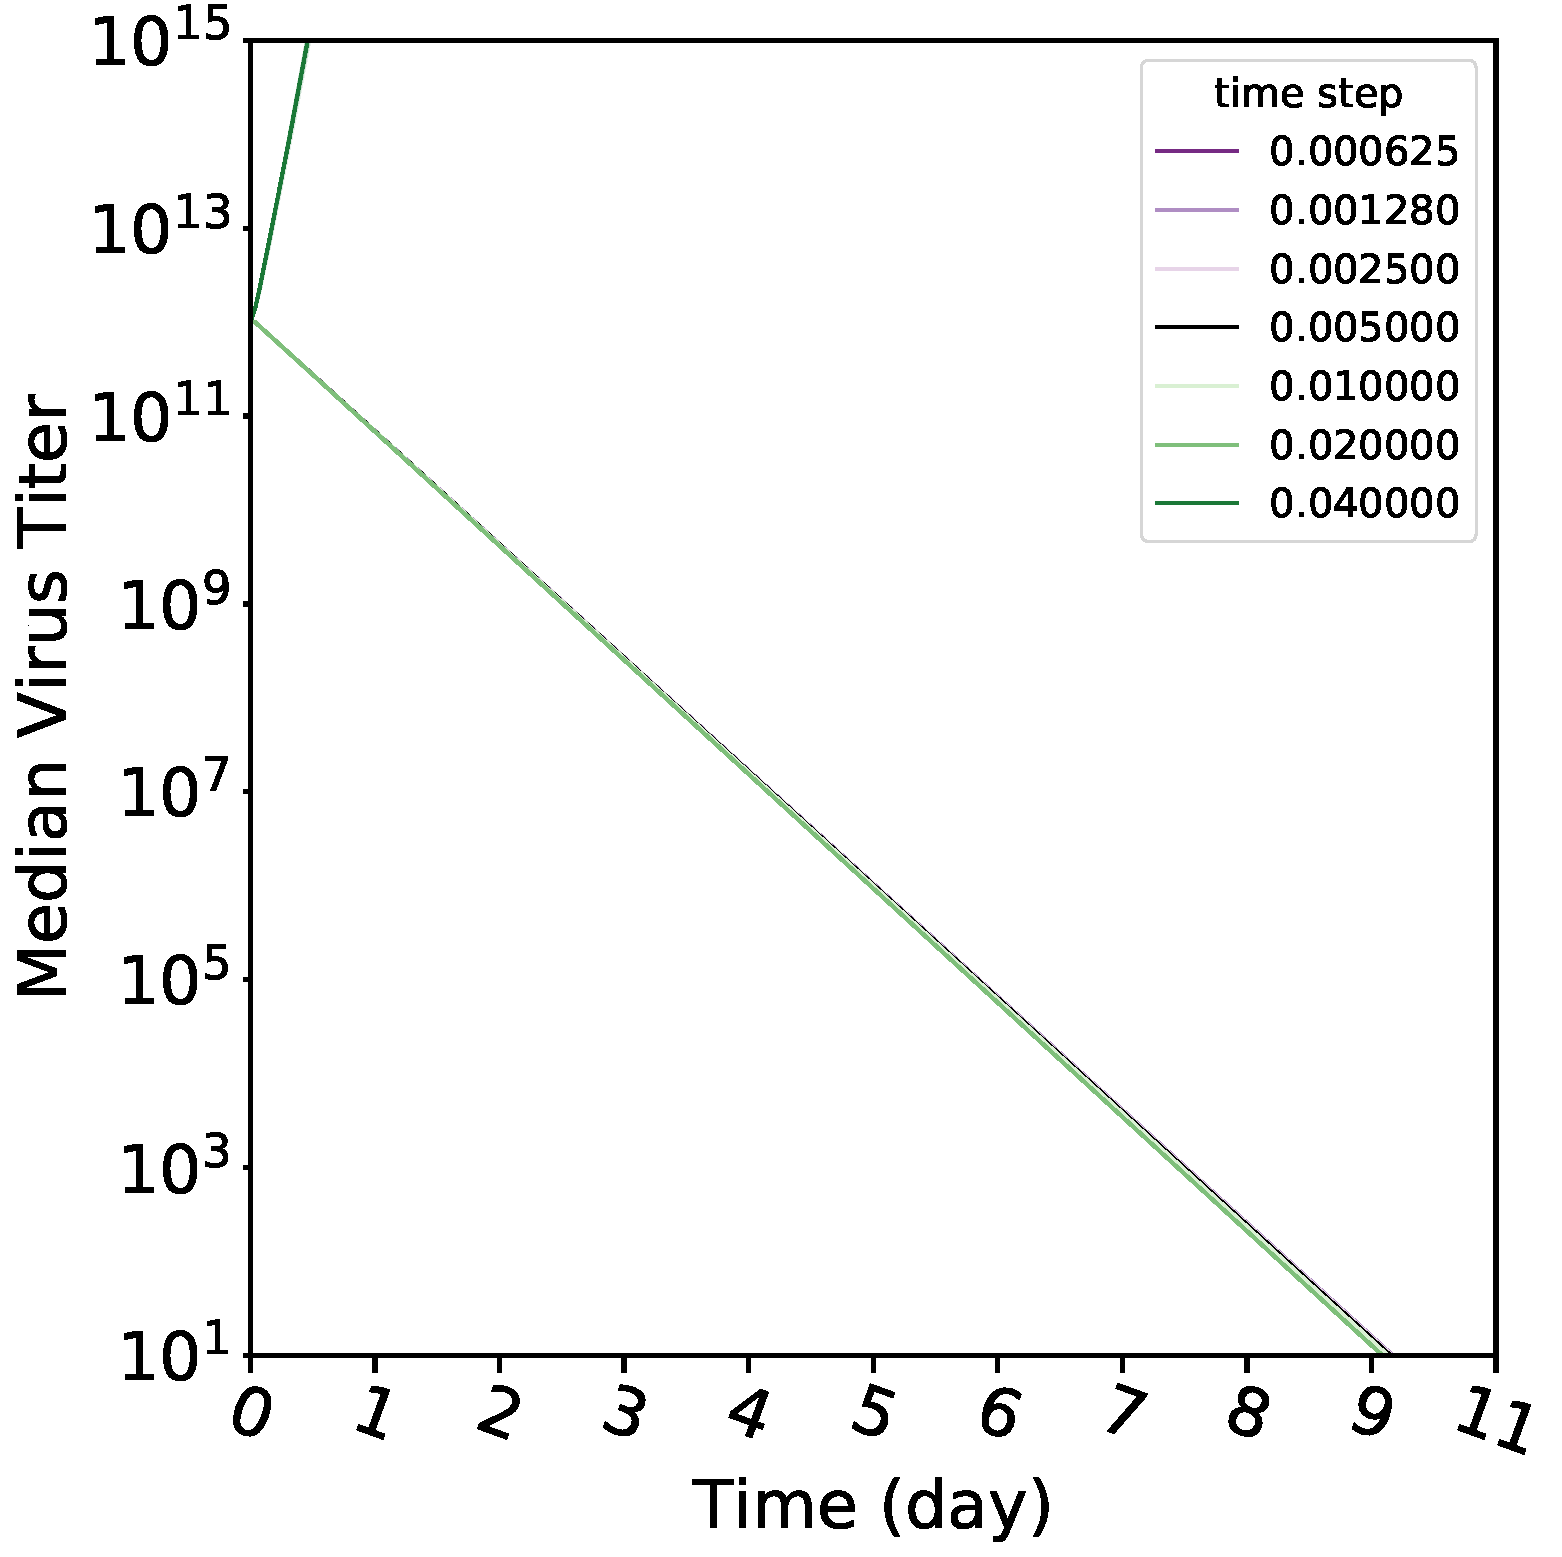
\includegraphics{Figures/Neither-InitialVirus-AllOnOne_Median_VirusVsTime.pdf}}}

\caption{The time step was varied to test the convergence of the model in time. A time step of 0.005 hr was chosen and a range around it was made by dividing or multiplying by 2 repeatedly. Seven values were used [0.000625, 0.00128, 0.0025, 0.005, 0.01, 0.02, 0.04]. The median curve of ten viral titer curves is shown for each time step. From left to right, curves of a viral infection exhibiting cell-free transmission initiated with infected cells; curves of a viral infection exhibiting cell-free transmission initiated with virus; and curves of virus without underlying cell infection. \label{fig:ViralTiterCurves}}
\end{figure}

%In figure \ref{fig_AspectGraphs} we explored the different viral titer curves further by plotting the measurable characteristics mentioned in section \ref{Viral_transmission} for each time step. We see very little change in any of the measured quantities until we reach the largest time step. \color{blue} I need to say something about the aspect graphs but I'm not sure what to say. \color{black} \color{red} I think we should take out this figure. It really doesn't add much. Leave it for the thesis.\color{black}

%\begin{figure}
%\captionsetup[subfigure]{aboveskip=-1pt,belowskip=1pt}
%\centering
%\begin{minipage}{\linewidth}
%    \centering

%    \fbox{\parbox{\textwidth}{\vspace{-1em}
%    \begin{multicols}{3}
%        \centering

%        Initial Cell

%        Initial Virus

%        Only Virus
%    \end{multicols}
%    \vspace{-1em}}}

%    \vspace{0.5em}

%    \begin{subfigure}[b]{0.3\linewidth}
%        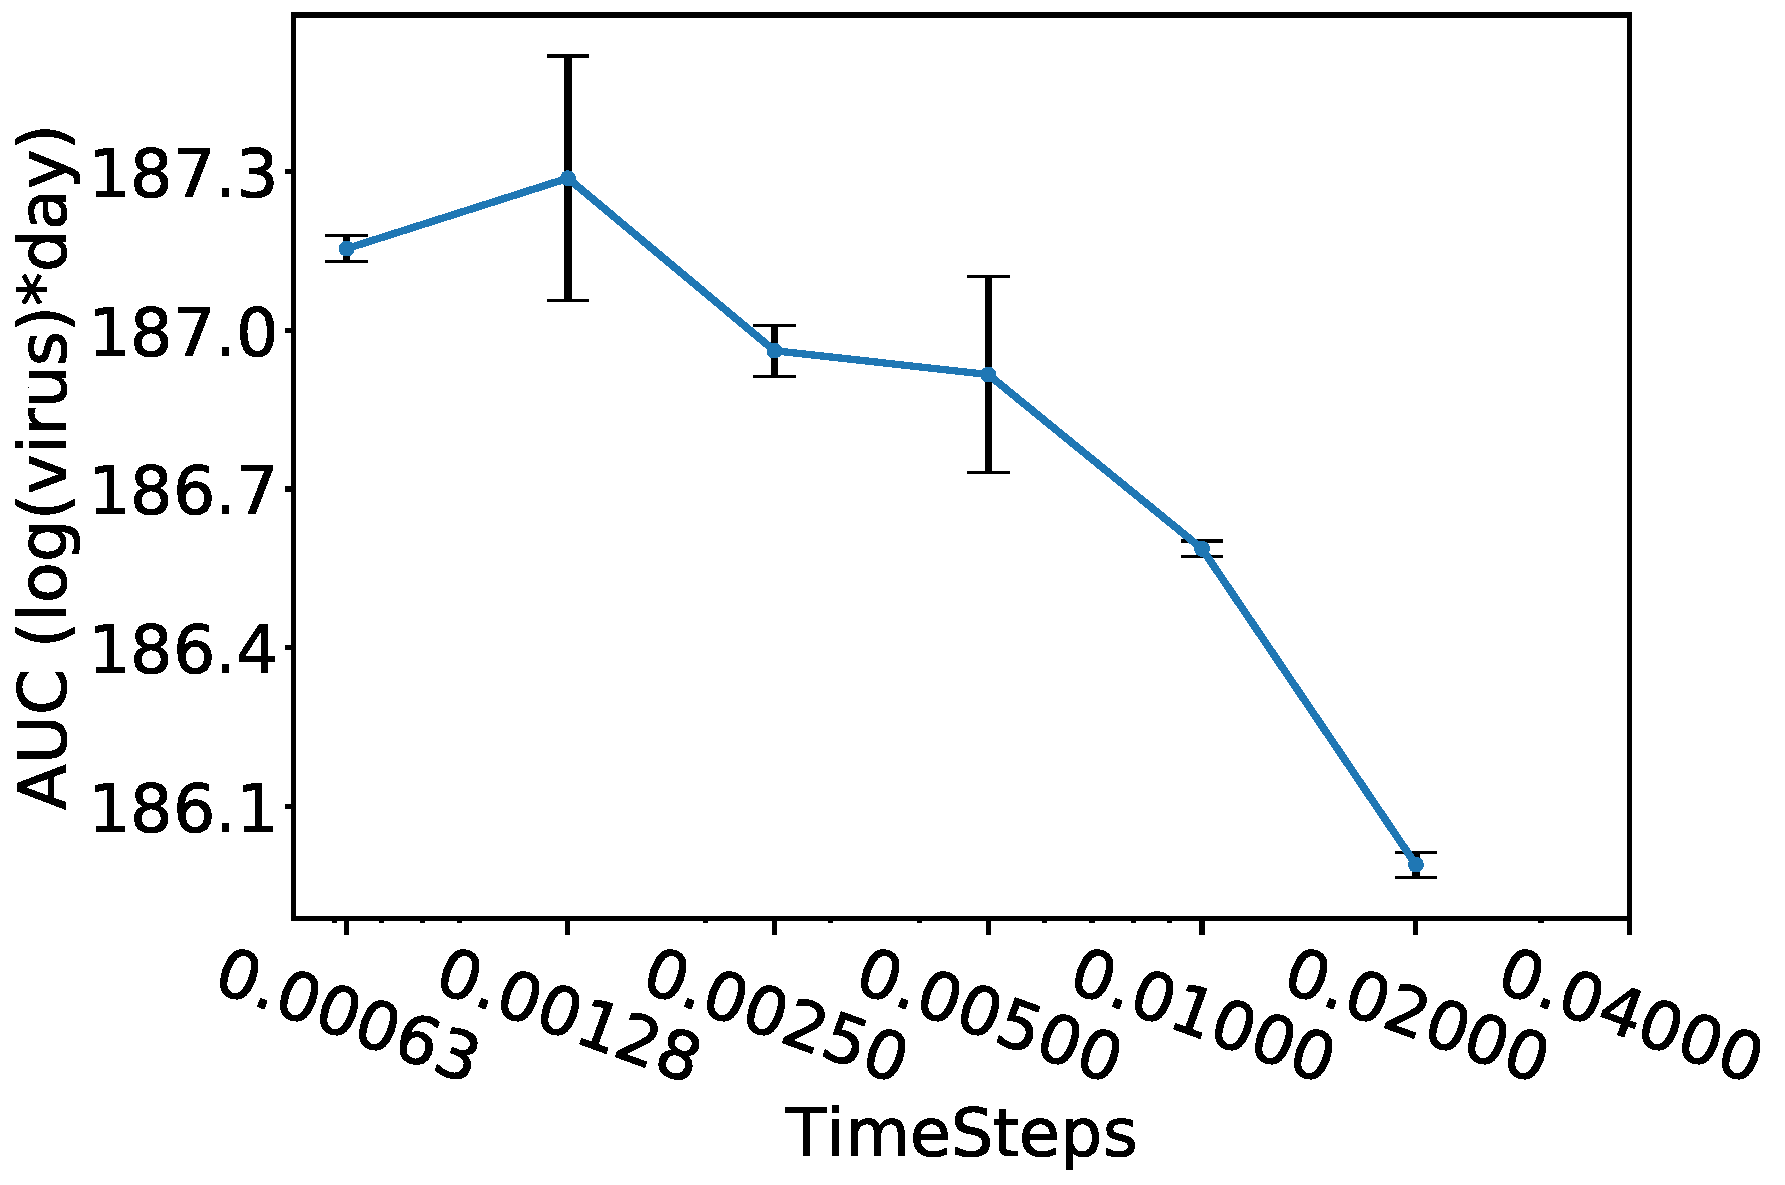
\includegraphics[width=\linewidth]{Figures/Cellfree-InitialCell-Runs_Graphs/AUC.pdf}
%        \caption{}
%        \label{fig:Peak_virus_of_both_transmission_modes}
%    \end{subfigure}
%    \begin{subfigure}[b]{0.3\linewidth}
%        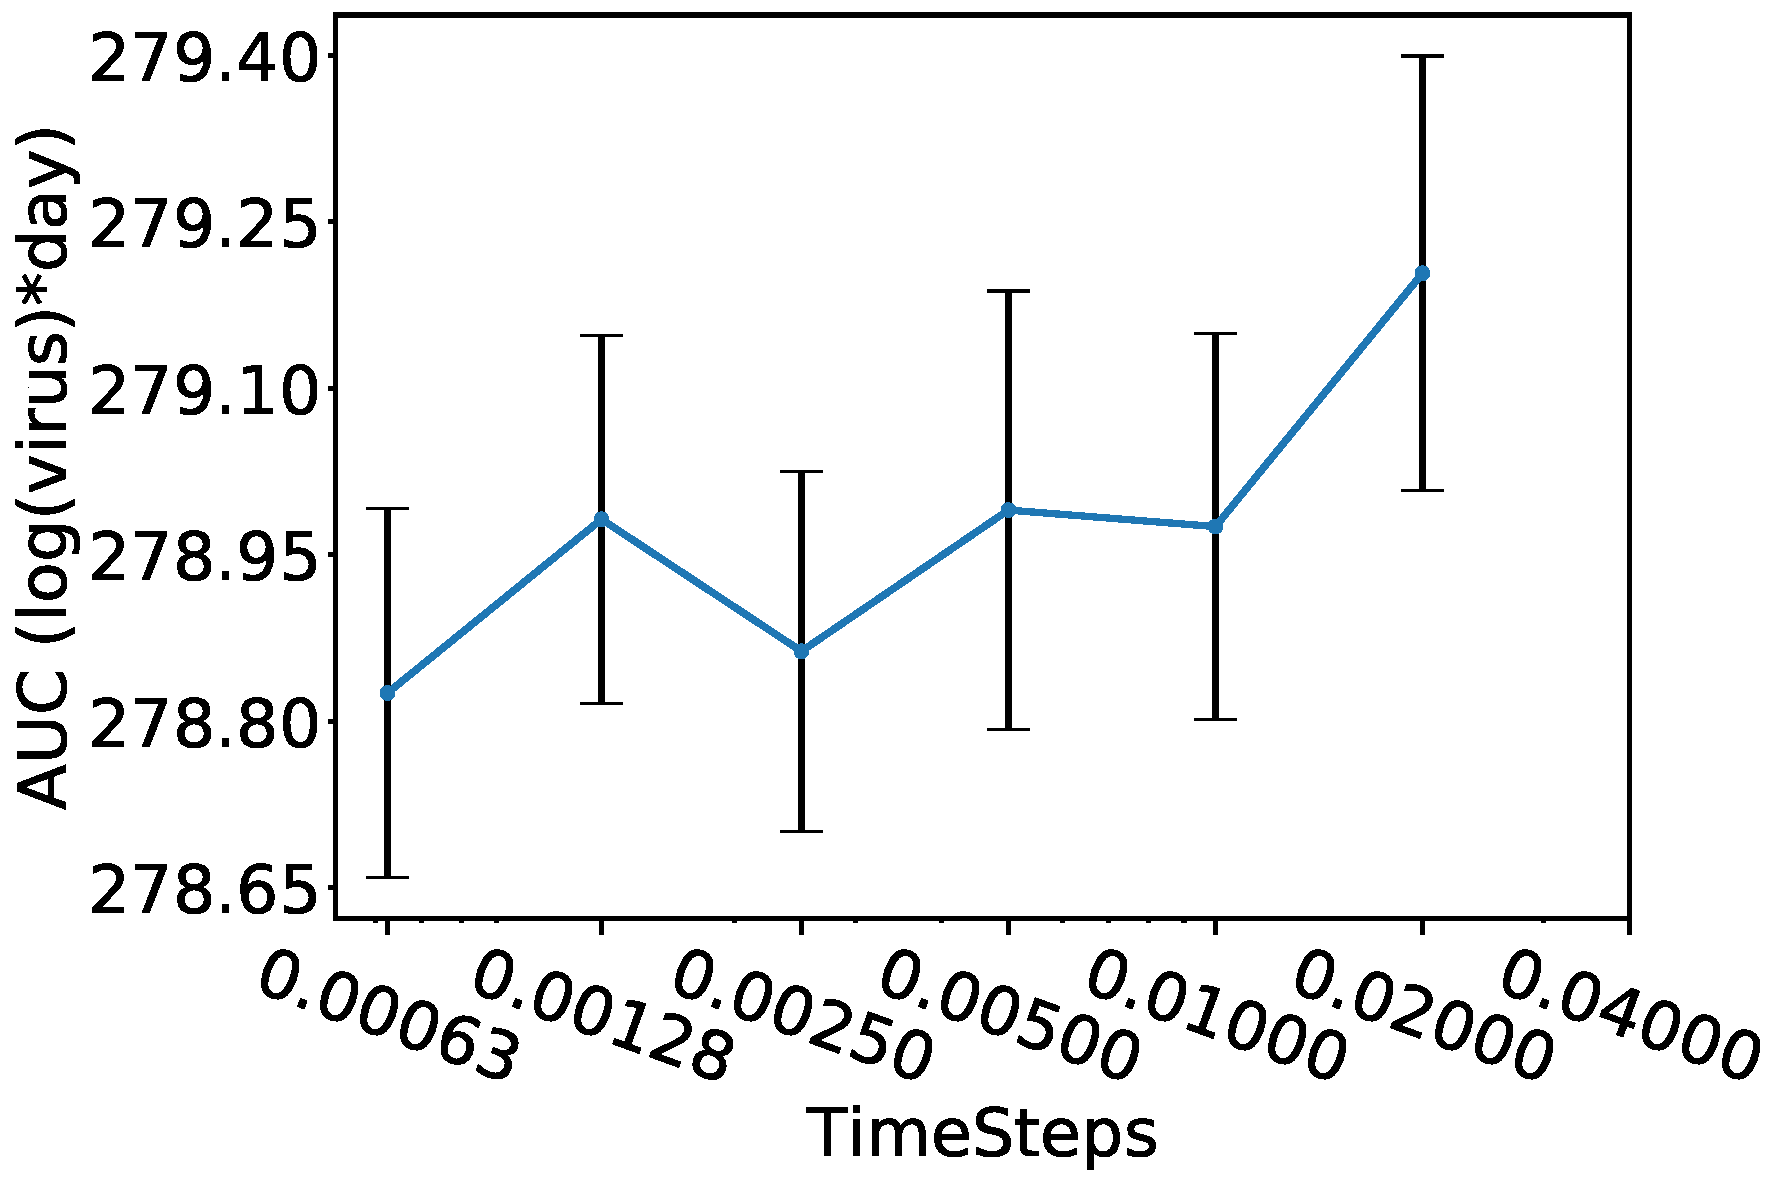
\includegraphics[width=\linewidth]{Figures/Cellfree-InitialVirus-Runs_Graphs/AUC.pdf}
%        \caption{}
%        \label{fig:Peak_virus_of_both_transmission_modes}
%    \end{subfigure}
%    \begin{subfigure}[b]{0.3\linewidth}
%        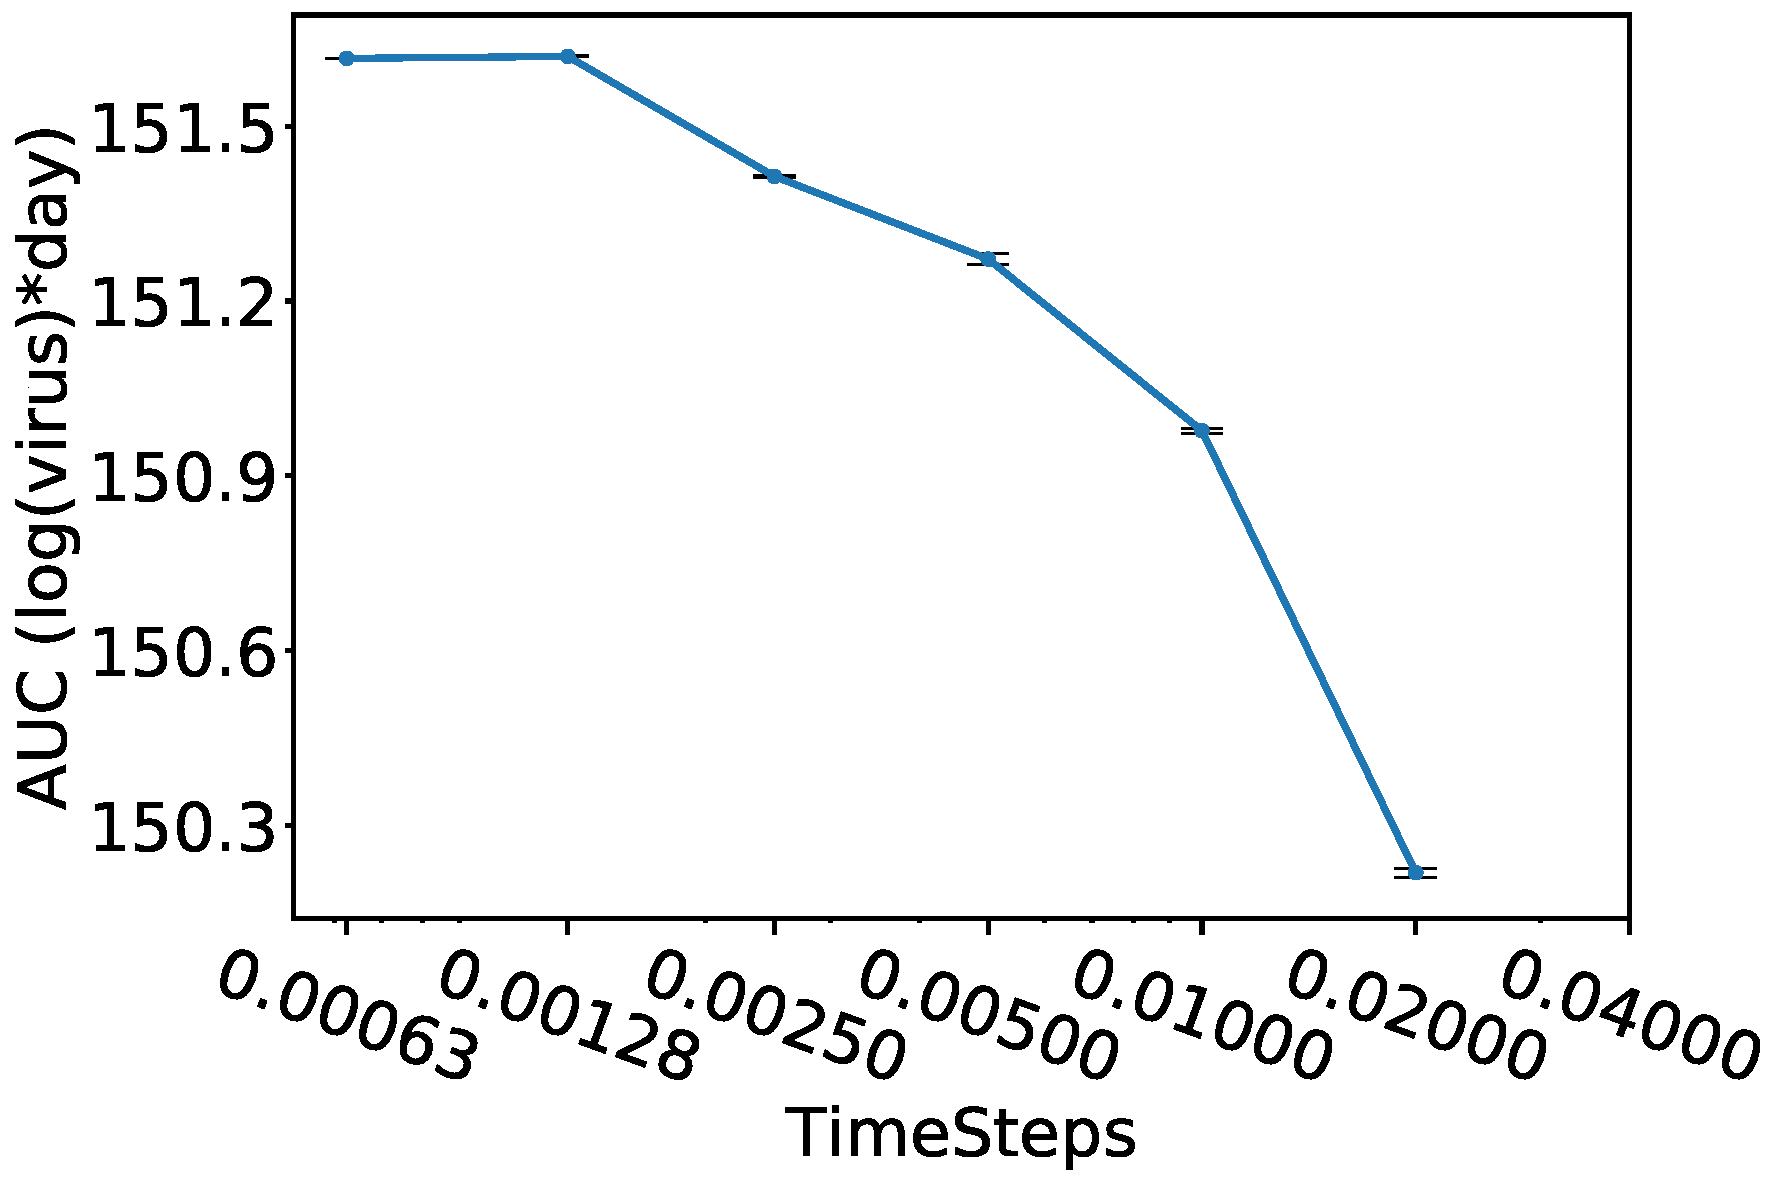
\includegraphics[width=\linewidth]{Figures/Neither-InitialVirus-Runs_Graphs/AUC.pdf}
%        \caption{}
%        \label{fig:Peak_virus_of_both_transmission_modes}
%    \end{subfigure}

%    \begin{subfigure}[b]{0.3\linewidth}
%        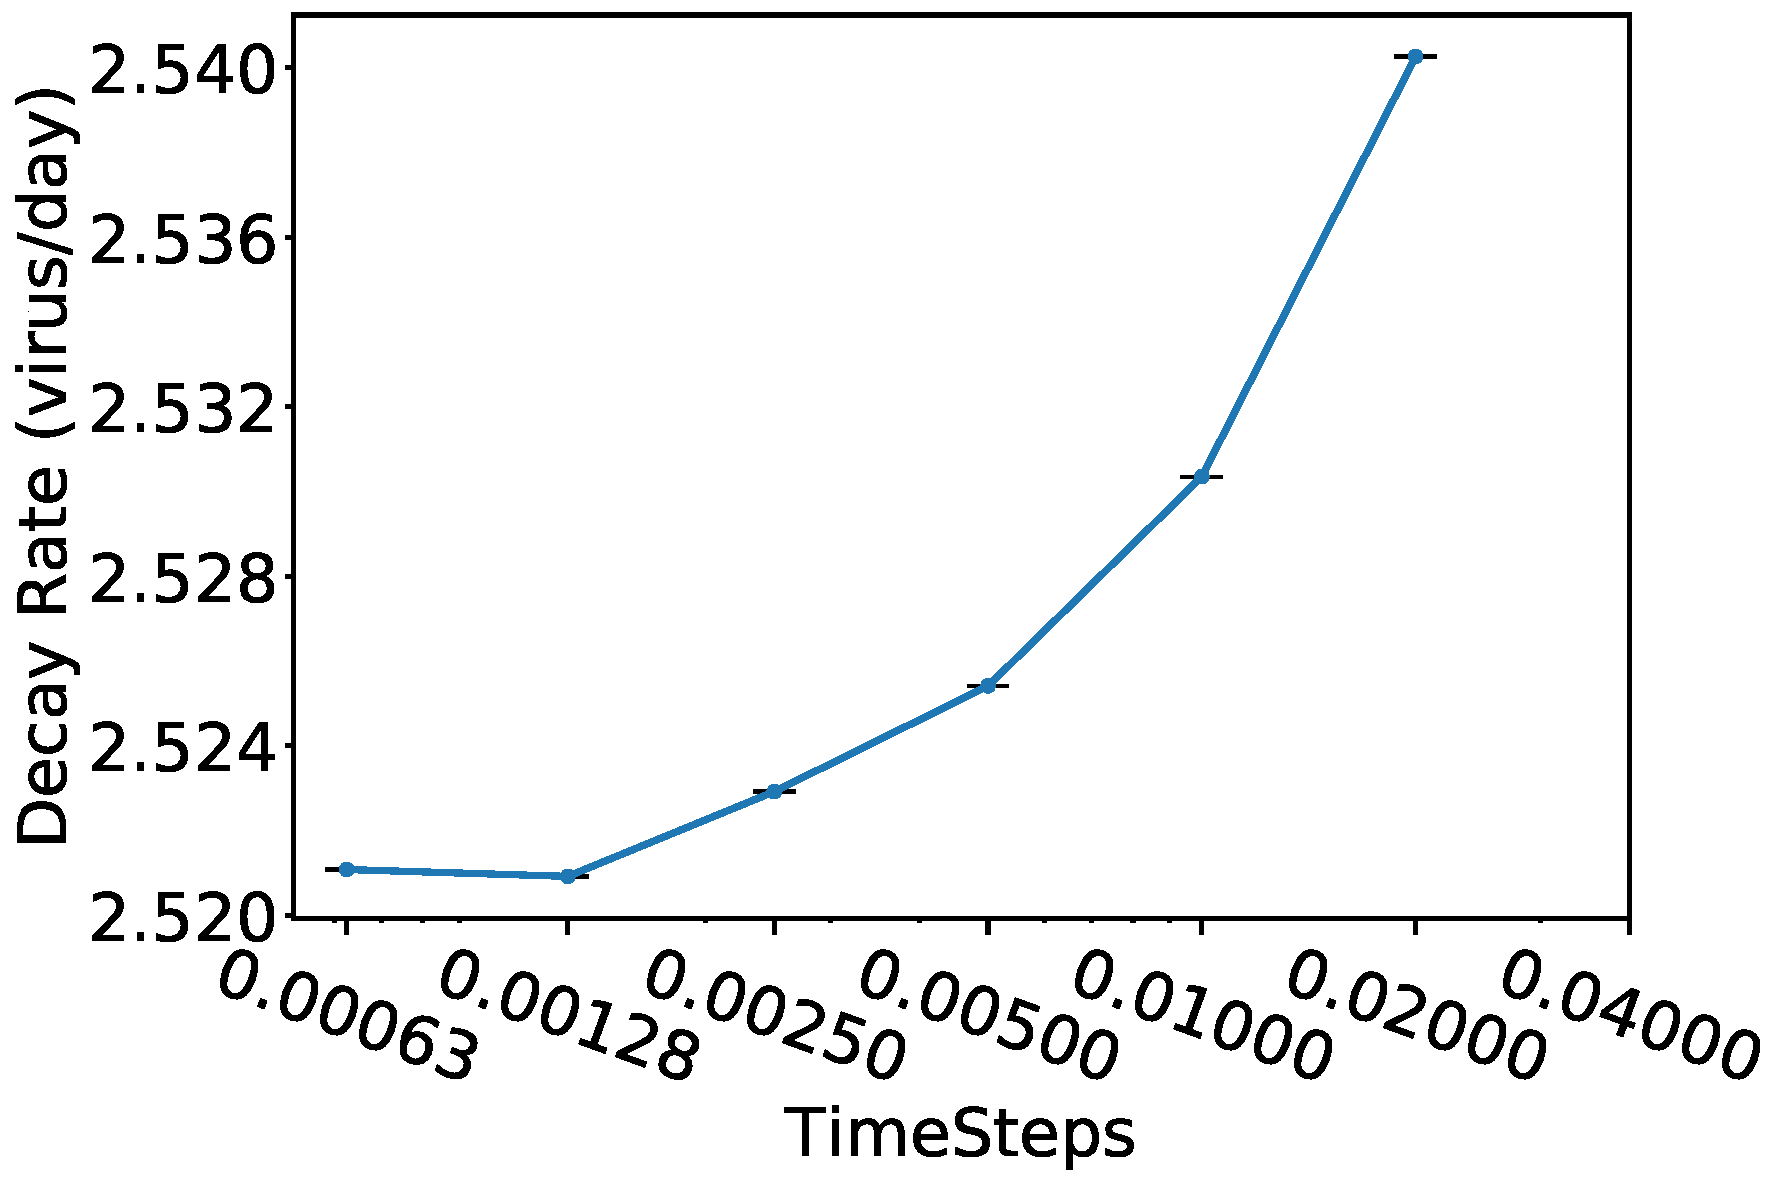
\includegraphics[width=\linewidth]{Figures/Cellfree-InitialCell-Runs_Graphs/DownSlope.pdf}
%        \caption{}
%        \label{fig:Peak_time_of_both_transmission_modes}
%    \end{subfigure}
%    \begin{subfigure}[b]{0.3\linewidth}
%        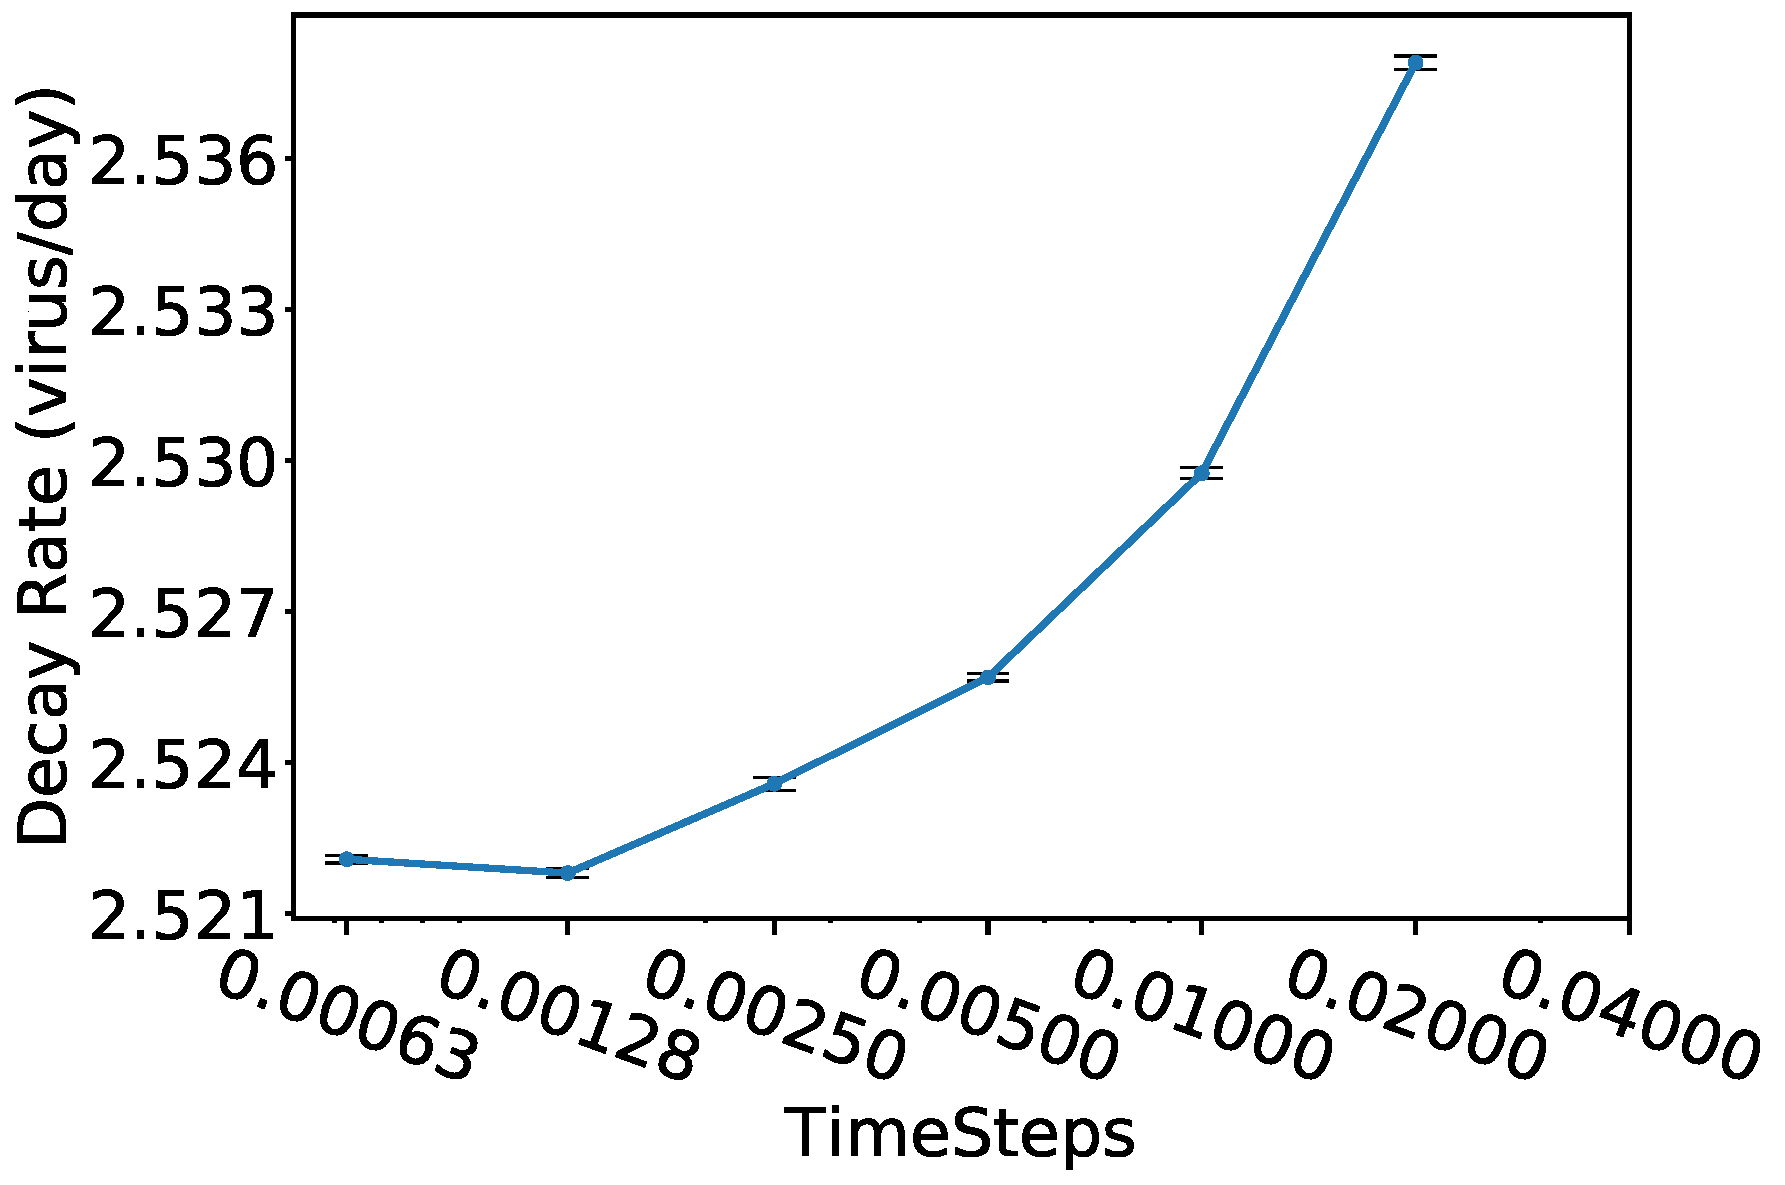
\includegraphics[width=\linewidth]{Figures/Cellfree-InitialVirus-Runs_Graphs/DownSlope.pdf}
%        \caption{}
%        \label{fig:Peak_time_of_both_transmission_modes}
%    \end{subfigure}
%    \begin{subfigure}[b]{0.3\linewidth}
%        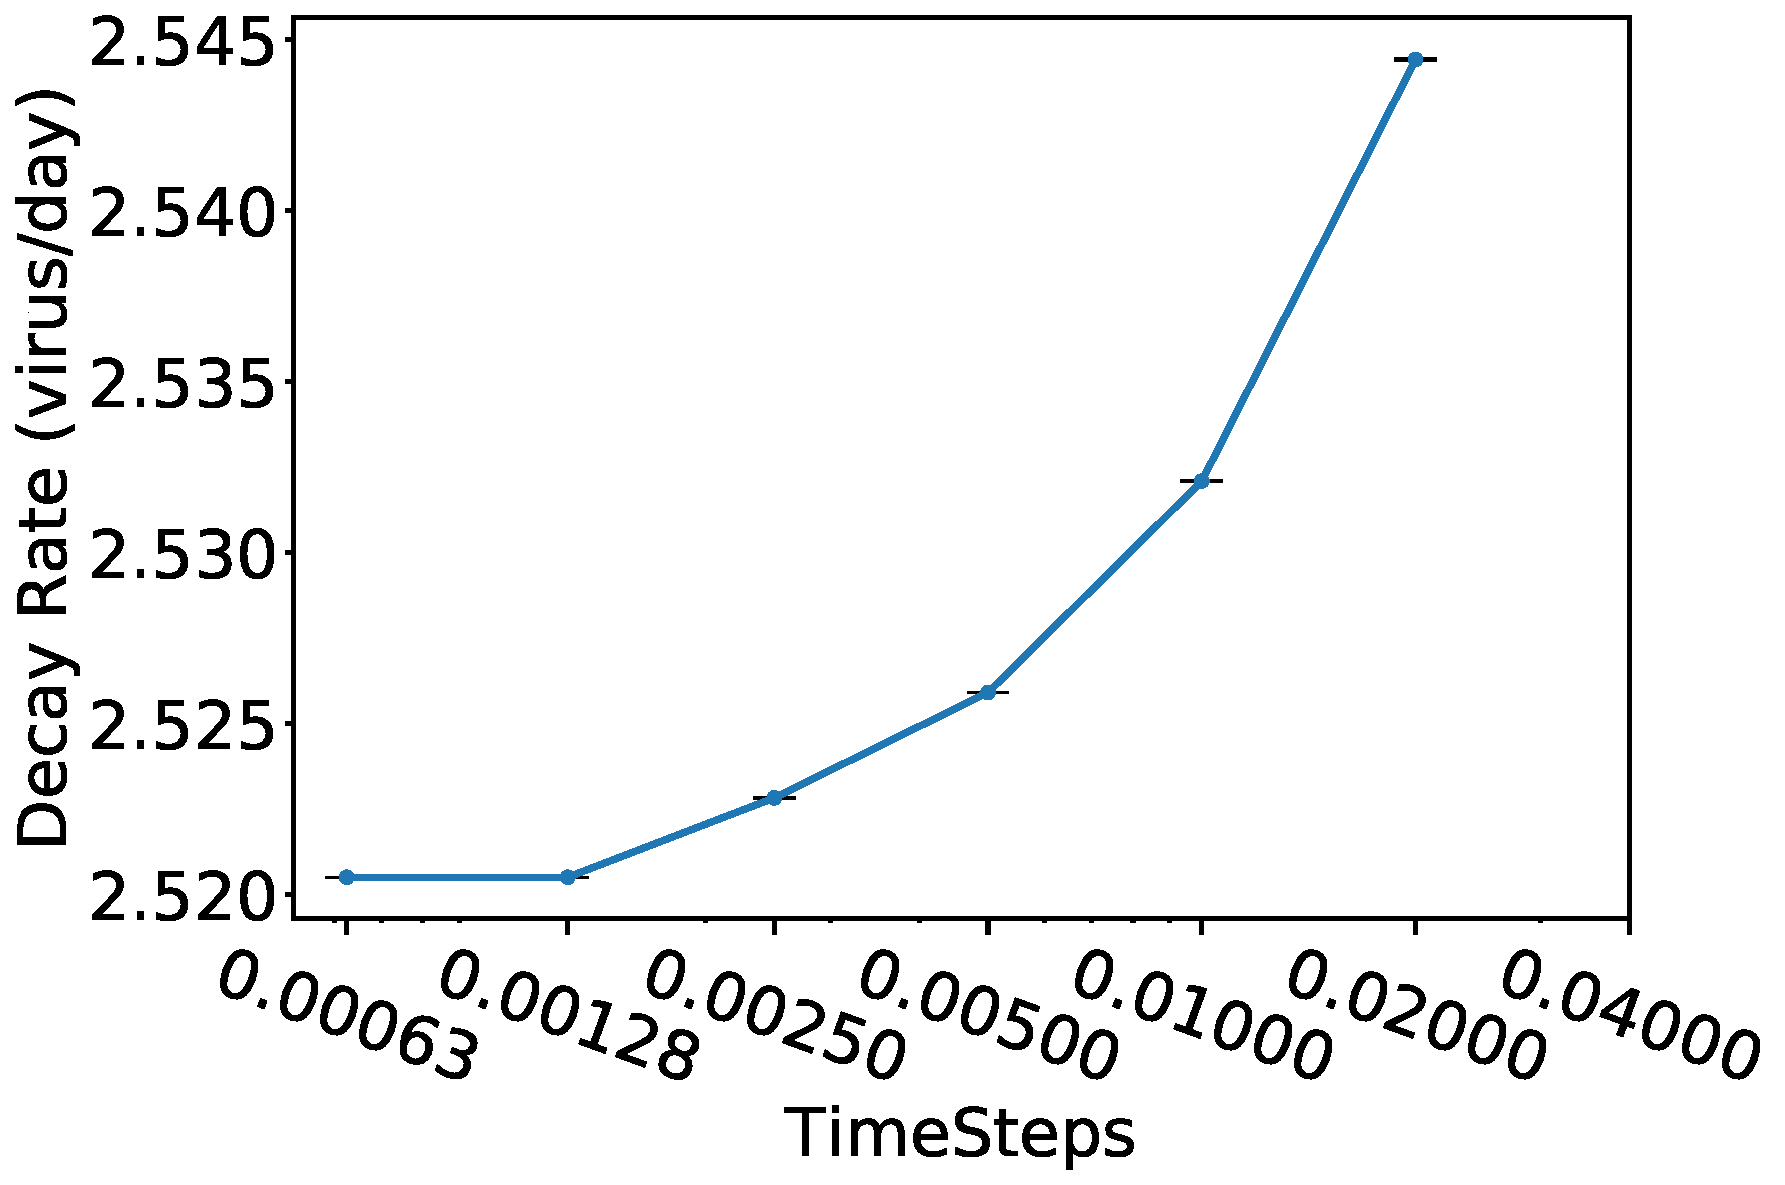
\includegraphics[width=\linewidth]{Figures/Neither-InitialVirus-Runs_Graphs/DownSlope.pdf}
%        \caption{}
%        \label{fig:Peak_time_of_both_transmission_modes}
%    \end{subfigure}

%    \begin{subfigure}[b]{0.3\linewidth}
%        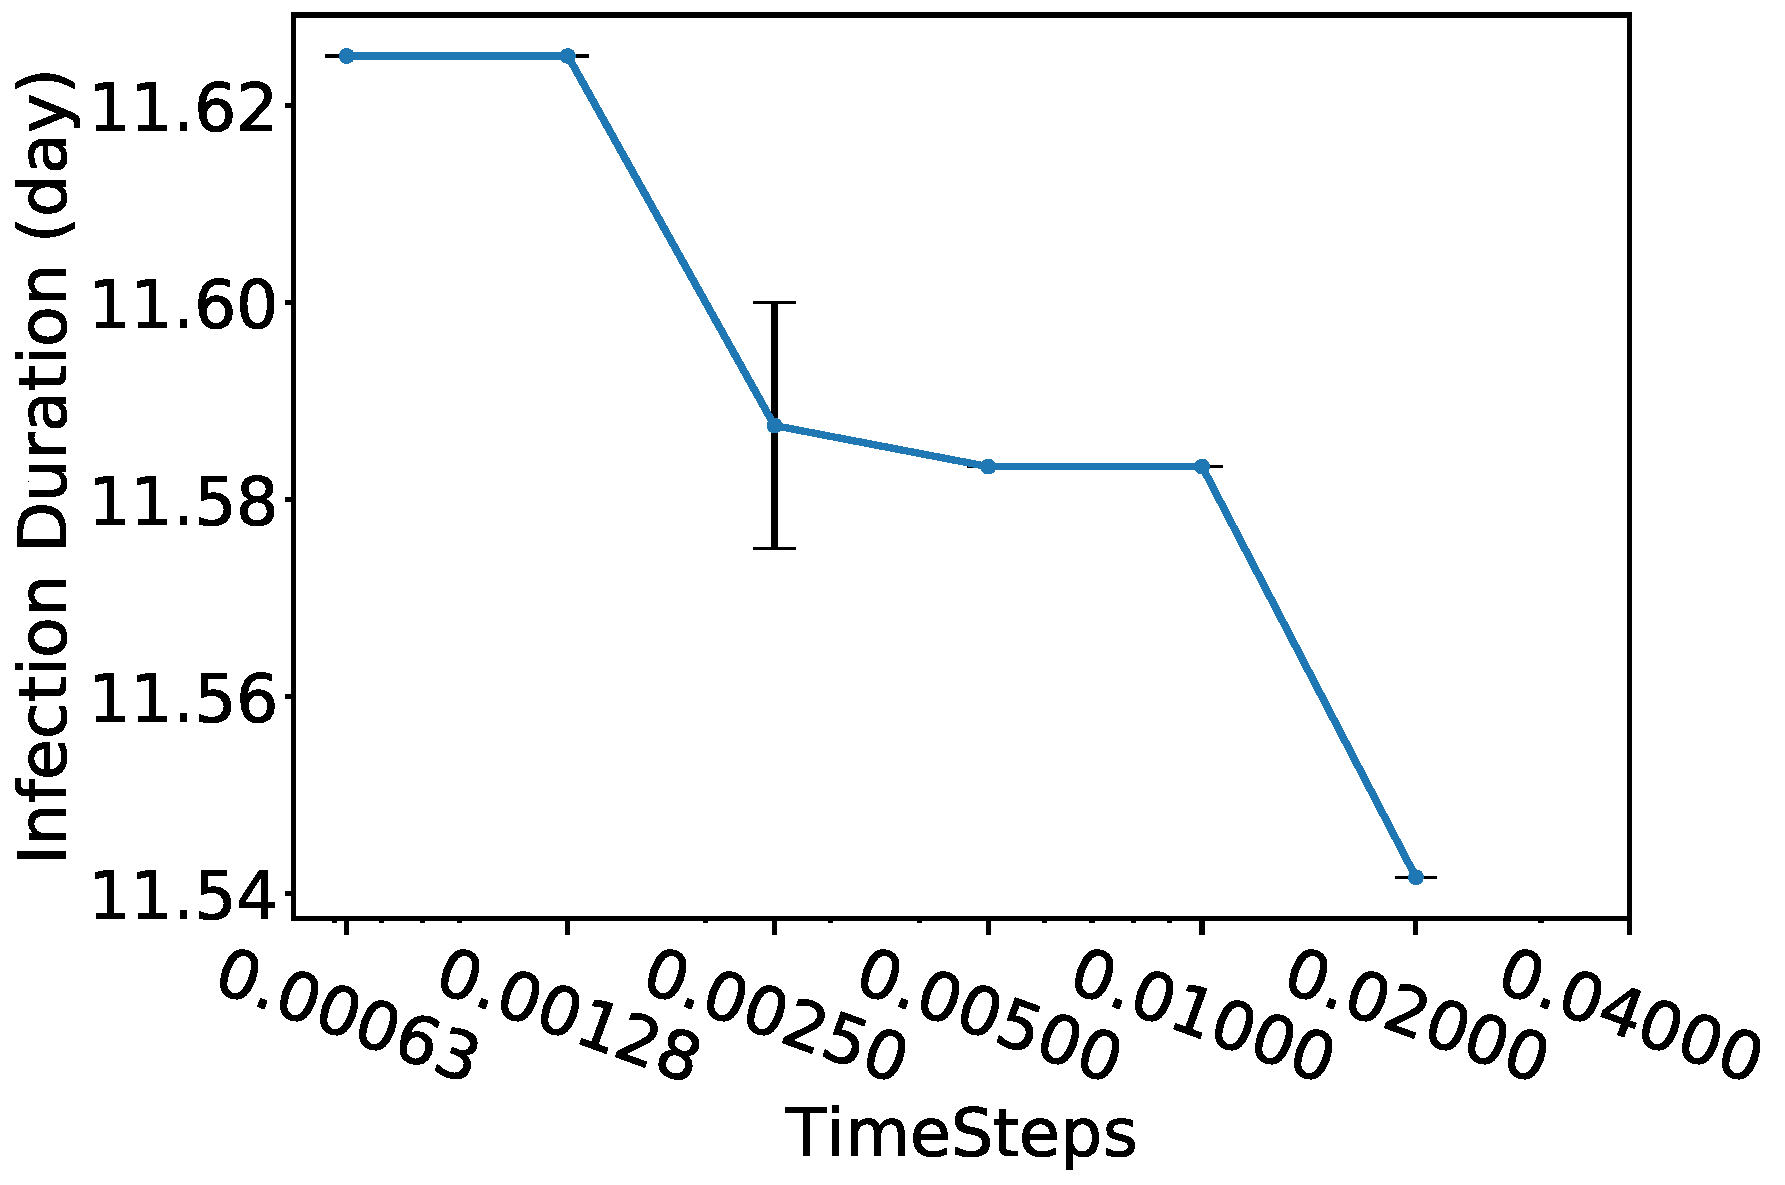
\includegraphics[width=\linewidth]{Figures/Cellfree-InitialCell-Runs_Graphs/InfectionDuration.pdf}
%        \caption{}
%        \label{fig:Growth_Rate_of_both_transmission_modes}
%    \end{subfigure}
%    \begin{subfigure}[b]{0.3\linewidth}
%        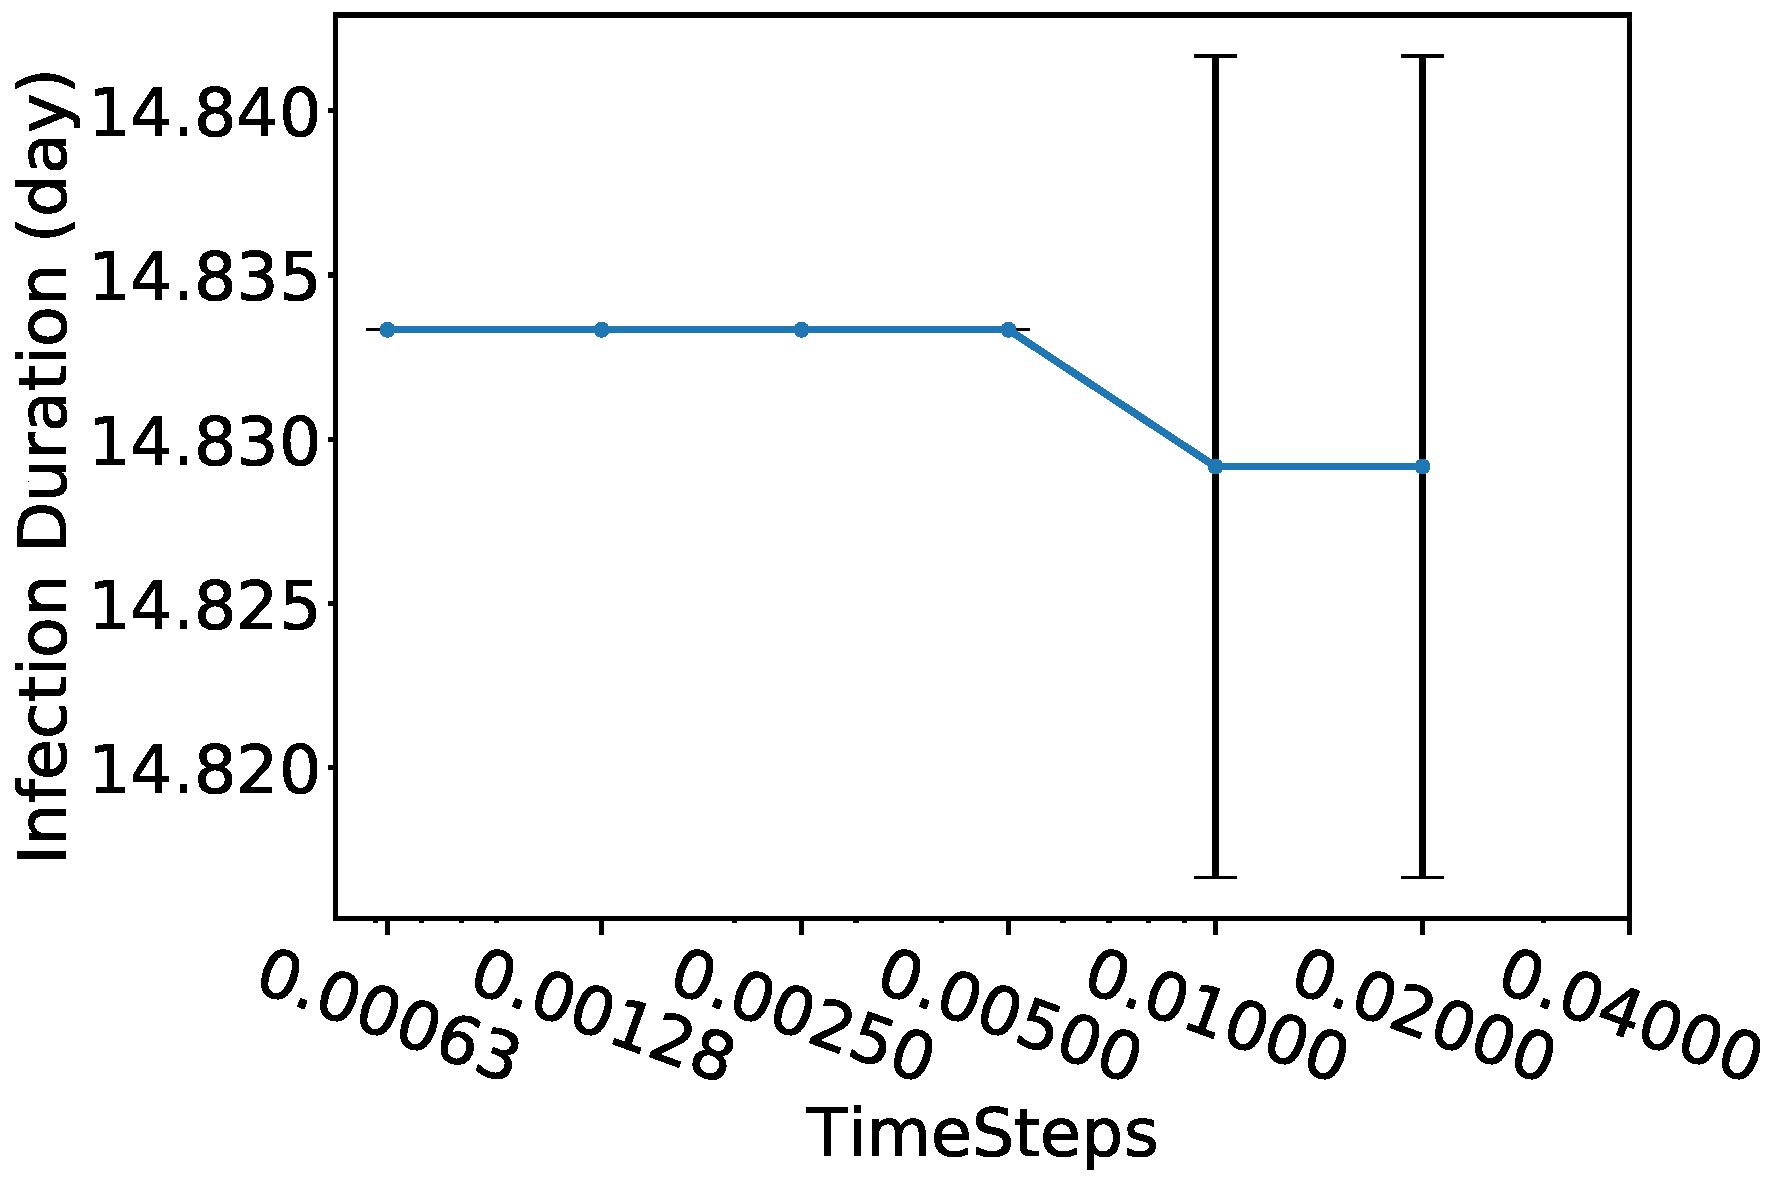
\includegraphics[width=\linewidth]{Figures/Cellfree-InitialVirus-Runs_Graphs/InfectionDuration.pdf}
%        \caption{}
%        \label{fig:Growth_Rate_of_both_transmission_modes}
%    \end{subfigure}
%    \begin{subfigure}[b]{0.3\linewidth}
%        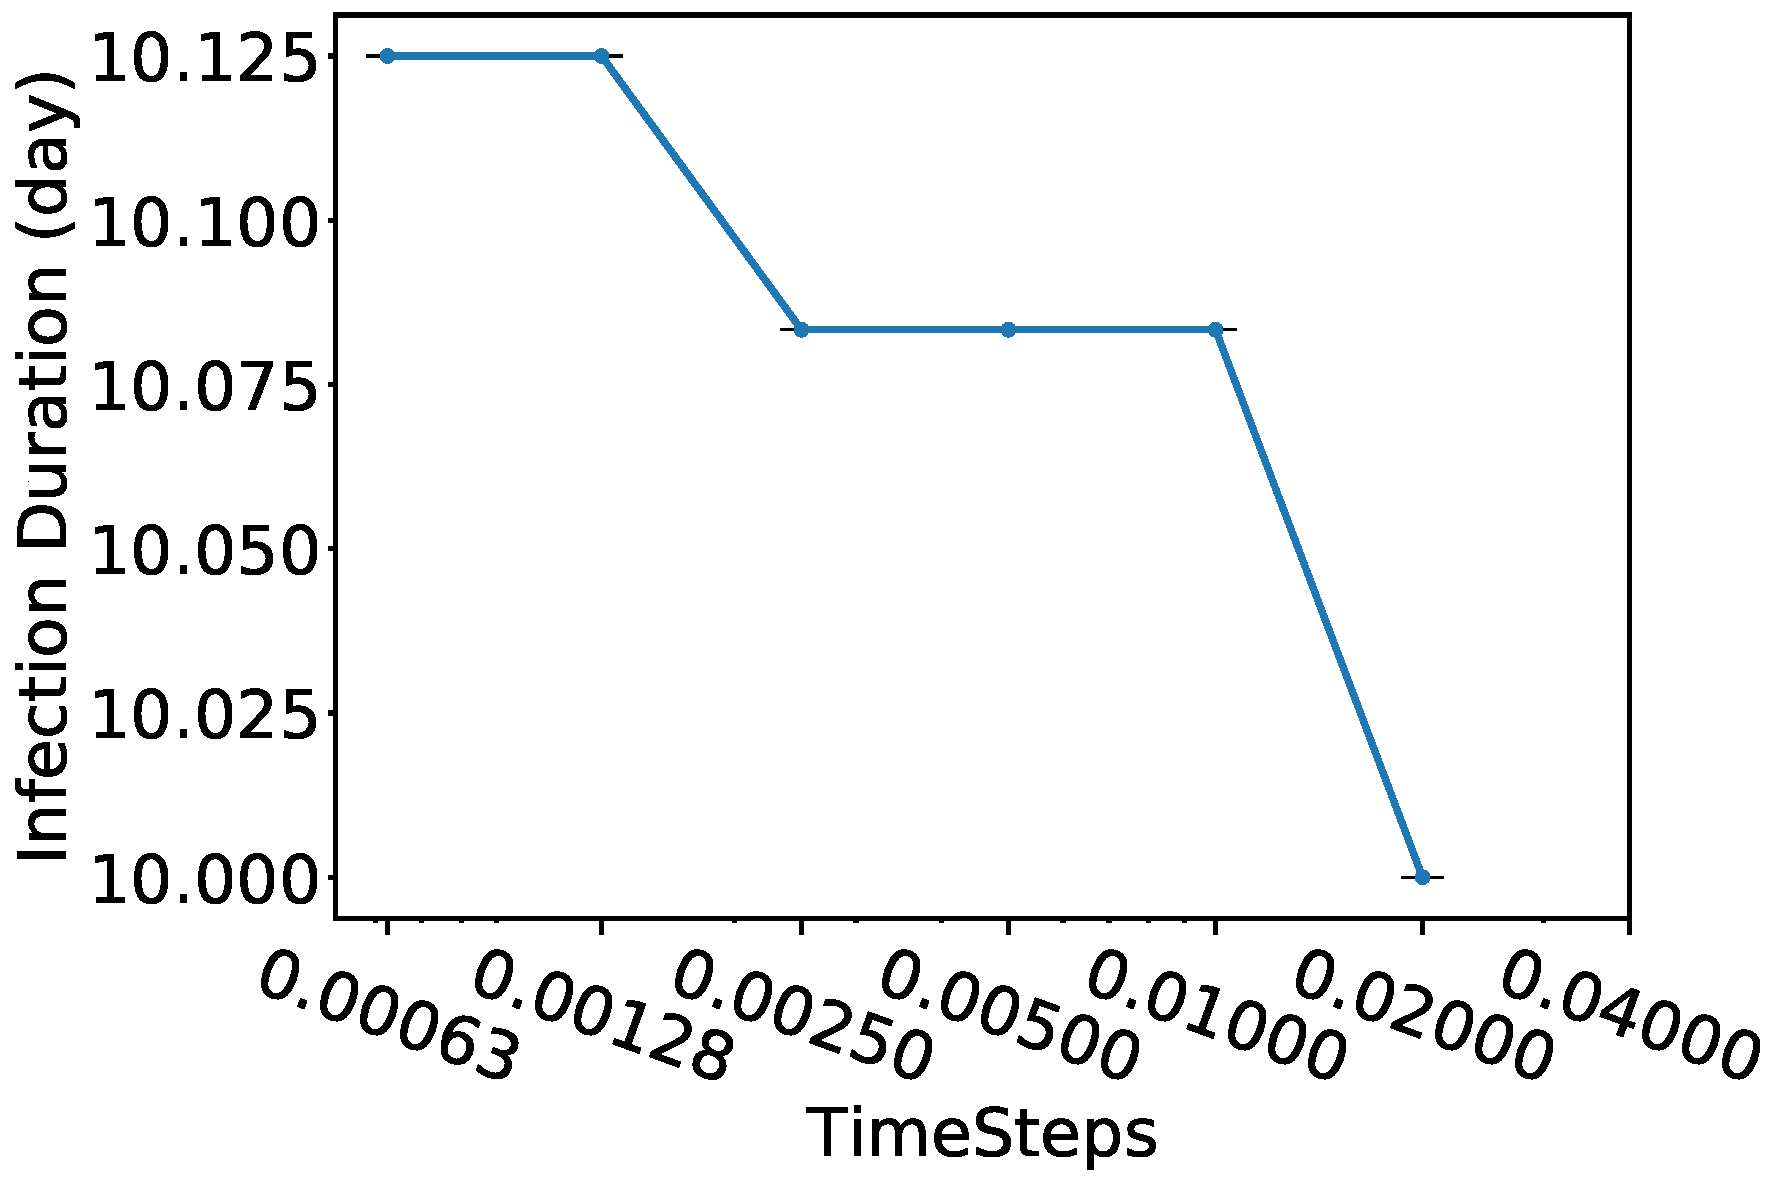
\includegraphics[width=\linewidth]{Figures/Neither-InitialVirus-Runs_Graphs/InfectionDuration.pdf}
%        \caption{}
%        \label{fig:Growth_Rate_of_both_transmission_modes}
%    \end{subfigure}


%    \begin{subfigure}[b]{0.3\linewidth}
%        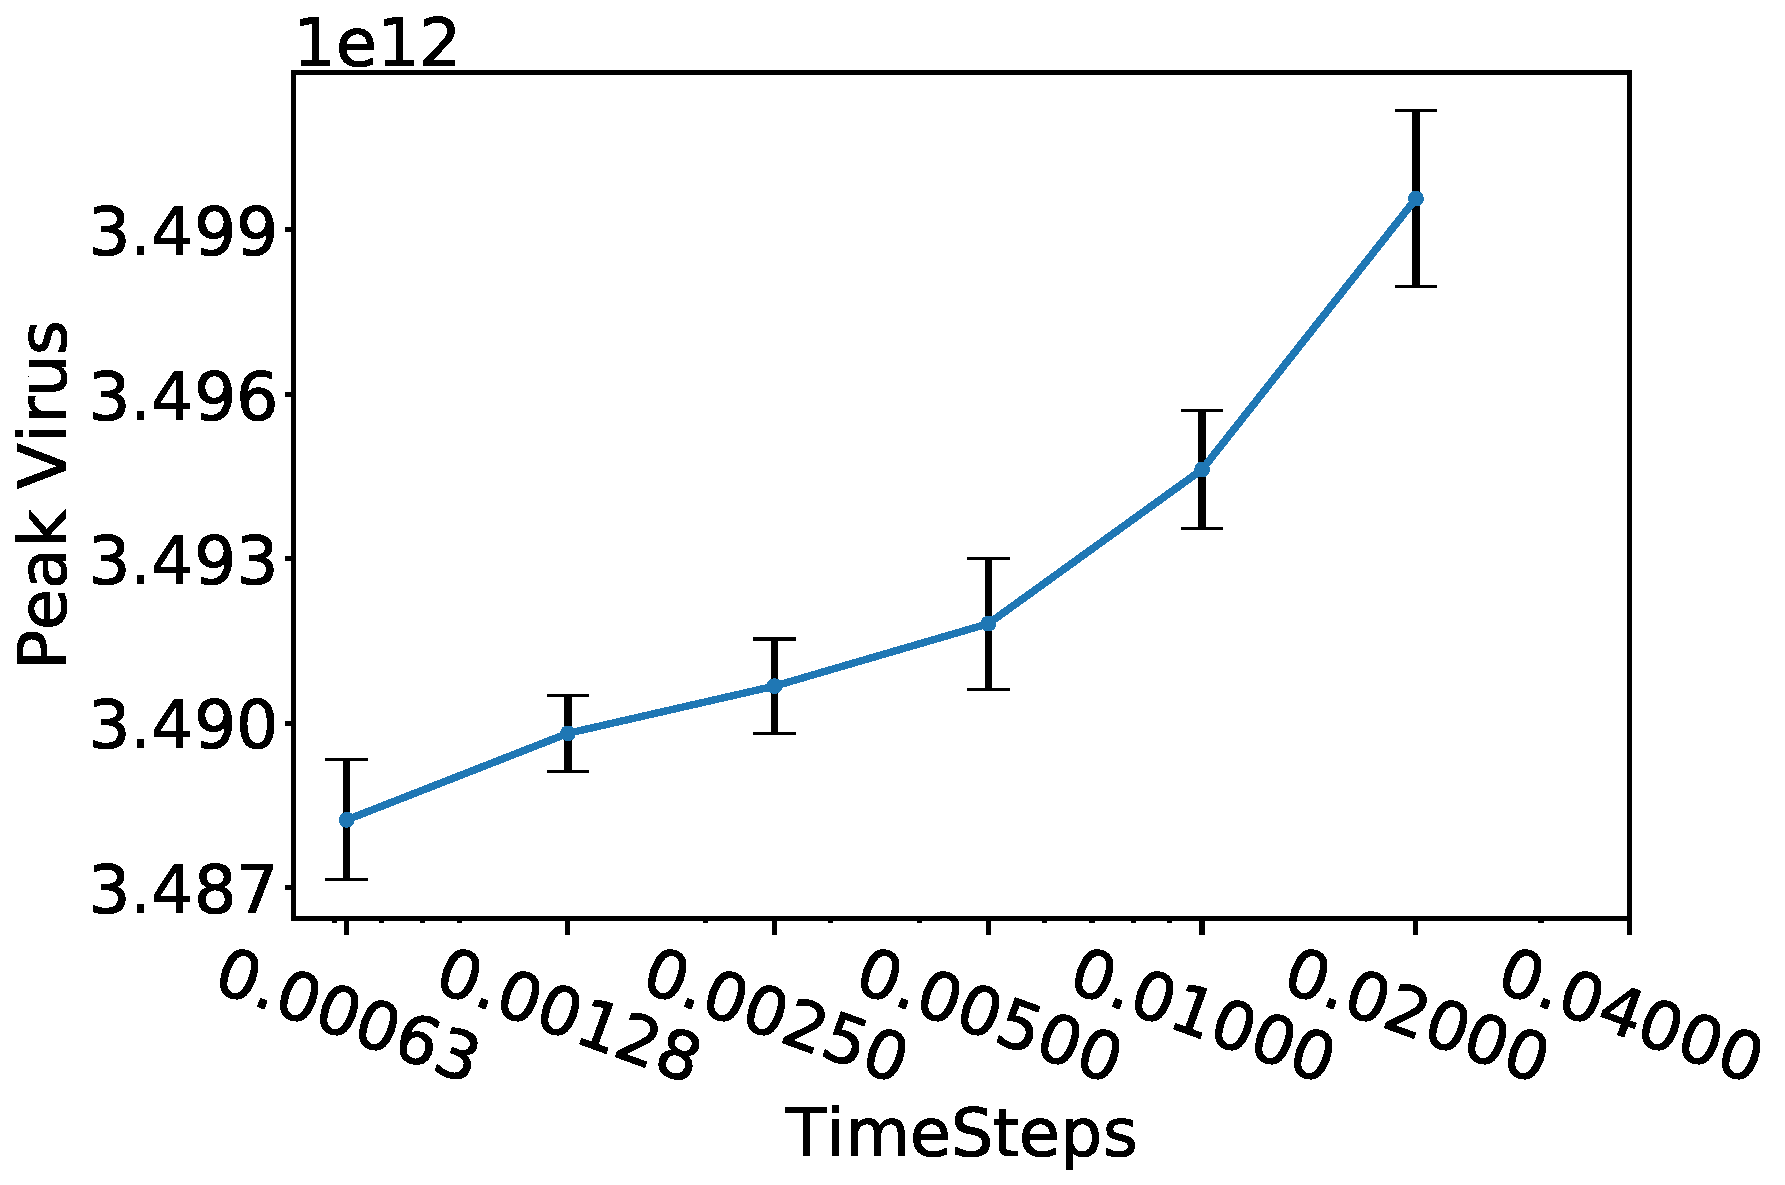
\includegraphics[width=\linewidth]{Figures/Cellfree-InitialCell-Runs_Graphs/PeakViralTiter.pdf}
%        \caption{}
%        \label{fig:Decay_Rate_of_both_transmission_modes}
%    \end{subfigure}
%    \begin{subfigure}[b]{0.3\linewidth}
%        \includegraphics[width=\linewidth]{Figures/Cellfree-InitialVirus-Runs_Graphs/PeakViralTiter.pdf}
%        \caption{}
%        \label{fig:Decay_Rate_of_both_transmission_modes}
%    \end{subfigure}
%    \begin{subfigure}[b]{0.3\linewidth}
%        \includegraphics[width=\linewidth]{Figures/Neither-InitialVirus-Runs_Graphs/PeakViralTiter.pdf}
%        \caption{}
%        \label{fig:Decay_Rate_of_both_transmission_modes}
%    \end{subfigure}

%    \begin{subfigure}[b]{0.3\linewidth}
%        \includegraphics[width=\linewidth]{Figures/Cellfree-InitialCell-Runs_Graphs/TimeofPeakViralTiter.pdf}
%        \caption{}
%        \label{fig:Decay_Rate_of_both_transmission_modes}
%    \end{subfigure}
%    \begin{subfigure}[b]{0.3\linewidth}
%        \includegraphics[width=\linewidth]{Figures/Cellfree-InitialVirus-Runs_Graphs/TimeofPeakViralTiter.pdf}
%        \caption{}
%        \label{fig:Decay_Rate_of_both_transmission_modes}
%    \end{subfigure}
%    \begin{subfigure}[b]{0.3\linewidth}
%        \includegraphics[width=\linewidth]{Figures/Neither-InitialVirus-Runs_Graphs/TimeofPeakViralTiter.pdf}
%        \caption{}
%        \label{fig:Decay_Rate_of_both_transmission_modes}
%    \end{subfigure}

%    \begin{subfigure}[b]{0.3\linewidth}
%        \includegraphics[width=\linewidth]{Figures/Cellfree-InitialCell-Runs_Graphs/UpSlope.pdf}
%        \caption{}
%        \label{fig:Decay_Rate_of_both_transmission_modes}
%    \end{subfigure}
%    \begin{subfigure}[b]{0.3\linewidth}
%        \includegraphics[width=\linewidth]{Figures/Cellfree-InitialVirus-Runs_Graphs/UpSlope.pdf}
%        \caption{}
%        \label{fig:Decay_Rate_of_both_transmission_modes}
%    \end{subfigure}
%    \begin{subfigure}[b]{0.3\linewidth}
%        \includegraphics[width=\linewidth]{Figures/Neither-InitialVirus-Runs_Graphs/UpSlope.pdf}
%        \caption{}
%        \label{fig:Decay_Rate_of_both_transmission_modes}
%    \end{subfigure}

%    \caption{Characteristics of the viral titer curves where measured for each of the seven time steps and the different scenerios.\label{fig_AspectGraphs}}
%\end{minipage}
%\end{figure}

%\clearpage
\subsection{Fitting the model to data}

We fit the model to experimental \emph{in vitro} data \cite{pinilla12} via minimization of the SSR. The initial condition of the simulations were: 501535 cells in the dish (similar to the number of cells in a typical 24-well plate \cite{Number_of_cells_in_a_dish_noauthor_useful_nodate}), 50 initial infected cells, and no virus in the dish. In figure \ref{fig_DataFit}, the median curve of ten simulations, using the best fit parameters, is plotted in dark blue alongside the data in green. Our best fit parameters are presented in Table \ref{tab_datafit_params}. Although the same data was used, some of our parameter estimates differ from those reported in Pinilla et al.\ \cite{pinilla12}. Our best fit $\tau_I$ is smaller than the $\tau_I = \SI{49}{\hour}$ reported by Pinilla et al., while our best fit $\tau_E$ is larger than the $\tau_E = \SI{6.6}{\hour}$ found by Pinilla et al., and the best fit $c$ is larger than $c = \SI{0.13}{\per\hour}$. Some of this discrepancy might be due to the inclusion of spatial effects in the ABM, but Pinilla et al.\ also used more data --- they used both a single cycle and multiple cycle experiment as well as viral RNA measurements --- to constrain the parameter estimates. All in all, the ABM/PDEM model can replicate the viral titer measurements of a typical infection via fitting where the fitting process uses standard packaged fitting algorithms and the computational time for fitting is less than 24 hours from inital guess to best fit.

\begin{table}
\centering
\caption{Best fit parameter values from fitting model to experimental data \cite{pinilla12}. \label{tab_datafit_params}}
\begin{tabular}{llc}
\hline
Parameter & Meaning & Value \\
\hline
$\beta$ & Infection rate & 54 $/\mathrm{h}$ \\
$p$ & Viral production rate & 3000 $/\mathrm{h}$ \\
$c$ & Viral clearance rate & 0.25 $/\mathrm{h}$ \\
$D$ & Diffusion coefficient & 2.2$\times 10^{-8}$ $\mathrm{m}^2/\mathrm{h}$ (fixed) \\
$\tau_E$ & Mean eclipse duration & 16 $\mathrm{h}$ \\
$\eta_E$ & Eclipse shape parameter & 30 (fixed) \\
$\tau_I$ & Mean infectious lifespan & 26 $\mathrm{h}$ \\
$\eta_I$ & Infectious shape parameter & 100 (fixed) \\
\end{tabular}
\end{table}

\begin{figure}
\centering
    \includegraphics[width=0.6\linewidth]{Figures/DataFit.pdf}
\caption{The ten simulated titer curves and corresponding median curve are plotted in blue. The experimental cell-free transmission data \cite{pinilla12} is plotted in green. The median curve has the minimal SSR with respect to the experimental data, when using the best fit parameters. The best fit parameters are shown in \ref{tab_datafit_params}. \label{fig_DataFit}}
\end{figure}

%\clearpage
\section{Discussion}

In this paper, we describe the construction of a hybrid ABM/PDEM model to investigate spatially extended viral infections. While the formulation of the model is similar to other ABM/PDEM models of viral spread \cite{beauchemin_simple_2005, bauer_agent-based_2009}, we have implemented our model to run on GPUs, vastly improving the simulation speed of these models. This allows for efficient replication of \emph{in vitro} infections with a realistic number of cells. This will help lead to a better understanding of virus-cell dynamics \emph{in vitro} \cite{blahut21}, but could also help realize the goal of simulating infections \emph{in vivo} \cite{laubenbacher21}. The faster simulations also allowed us to use standard ODE model-fitting techniques to fit this model to experimental data, making it possible to quickly parameterize these models to reproduce dynamics of different viruses. Previously, researchers have had to develop other techniques to help speed up fitting of ABMs to experimental data, including reducing the sampled parameter space \cite{li17}, and mapping of ABM outputs to simpler functions \cite{tong_development_2015, read16}. These techniques coupled with simulation of ABMs on GPUs could potentially allow for real-time parameter estimation of models for use in patient care. This is particularly useful for a novel pandemic virus that can be simulated such that trial runs of test drugs can be performed and viral infection severity for a patient can potentially be predicted. 


\section{Covid Paper Results}

Fig.\ \ref{curves} shows the viral titer curves for different MOI of SARS-CoV-2, where the darker line for each color shows the curve of median values and the lighter colored lines are the 100 individual simulations. Note that for most MOI, there is very little variation between simulations once the viral titer is large. The exception is the lowest MOI of 10$^{-5}$ where there is more variation in the exact trajectory of the viral load. We see some obvious shifts in the viral titer curve as the MOI increases. For high MOI, the viral titer curve reaches its peak very quickly, with lower MOIs moving the peak farther out in time. The peak also becomes broader and lower as the MOI becomes lower, suggesting longer infection durations, but with lower viral loads.
\begin{figure}[!h]
\begin{center}
\resizebox{0.6\textwidth}{!}{\includegraphics{Figures/Covid_AllOnOne_Median_VirusVsTime}}
\caption{Viral loads for infections initiated with different MOI. Dark lines of each color indicate the viral load curve using the median of 100 simulations, while the lighter colored lines show the viral load kinetics for each individual simulation. The dashed line indicates the threshold of detection used to calculate infection duration. \label{curves}}
\end{center}
\end{figure}

For a more quantitative assessment, we measure the characteristics described in Methods. The results are shown in Fig.\ \ref{results}, which shows peak viral load (top left), time of viral peak (top right), viral upslope (center left), AUC (center right), and infection duration (bottom) as functions of the MOI. The peak viral load increases with increasing initial inoculum, but it appears to reach a plateau as we near an MOI of 1. The time of peak, on the other hand, decreases with increasing initial inoculum, reaching a fixed small value at high MOI. There are real plateaus here since each cell will produce an average of $p\tau_I$ viral particles. At an MOI of 1, all cells are initially infected and will start producing virus at about the same time, meaning that all that virus is released almost simultaneously and there is no second cycle of infection. At slightly lower MOIs, most cells are initially infected, but some cells will be infected in a second or third cycle of infection, reducing the large burst of virus at one time, which causes a delay, reduction, and broadening in the peak. The upslope, or growth rate, of the viral titer curve increases as the MOI increases. This is also driven by the larger amount of virus being produced in the first cycle of infection as the MOI increases. Finally, the AUC and infection duration both decrease as the initial inoculum increases.  
\begin{figure}[!h]
\begin{center}
%\resizebox{0.48\textwidth}{!}{\includegraphics{Figures/CovidApectGraphs/PeakViralTitter}}
%\resizebox{0.48\textwidth}{!}{\includegraphics{Figures/CovidApectGraphs/TimeofPeakViralTitter}}
%\resizebox{0.48\textwidth}{!}{\includegraphics{Figures/CovidApectGraphs/New_UpSlope}}
%\resizebox{0.48\textwidth}{!}{\includegraphics{Figures/CovidApectGraphs/AUC}}
%\resizebox{0.48\textwidth}{!}{\includegraphics{Figures/CovidApectGraphs/InfectionDuration}}
\caption{Effect of initial inoculum on viral titer characteristics. The graphs show peak viral load (top left), time of viral peak (top right), viral upslope (center left), AUC (center right), and infection duration (bottom) as functions of MOI. \label{results}}
\end{center}
\end{figure}

%%%%%%%%%%%%%%%%%%%%%%%%%%%%%%%%%%%%%%%%%%
\section{Discussion}

Our study finds that initial viral inoculum does alter the viral time course by increasing the peak viral load, moving the peak earlier, increasing the viral upslope, and decreasing both AUC and infection duration, as the initial inoculum increases. It is not immediately clear what these changes in viral kinetics mean for the severity of the infection. Is it better to have a shorter infection, albeit with a higher viral peak, or a longer-lasting infection with a lower viral burden? One study compared viral loads in patients with mild and severe illness finding that the viral load time course in mild cases peaked earlier and at a lower peak viral load than in severe cases, although both time courses still had rather high viral loads at 25 days post symptom onset \cite{zheng20}. Since viral load in these patients was measured after they presented at a hospital, there is also no way to link particular features of the viral time course to the initial inoculum. Other observational studies that have attempted to investigate links between viral load and disease severity have taken a limited number of viral load measurements, often well after the peak of the infection \cite{liu20, liu20imm,to20}, making it impossible to assess the full time course of the viral load, and any correlations to initial inoculum. An alternative to observational studies in patients is to investigate inoculum dose-response of SARS-CoV-2 in animals, as suggested in \cite{little20}. Such animal studies in conjunction with mathematical modeling studies will help provide a clearer picture of the role of initial inoculum in determining viral time course and disease severity.


